\chapter{Frontend Structure}
\label{chapter:frontend}

\todo[inline]{intro}

\section{Home Page}

\todo[inline]{todo}

\section{Visualization Terminology}

The explanations provided in the present documentation as well as in the info texts in the visualization use terminology and concepts from information visualization.
We strove to make these texts as accessible as possible to a wider audience, but some basic understanding of the concepts used is still required.
Here, we introduce the terms we used, and explain the visualization types.

\subsection{Interactive Visualization}

Card et al.~\cite{Card_1999} formalized the \emph{data visualization pipeline}\footnote{See \url{https://infovis-wiki.net/wiki/Visualization_Pipeline}} in 1999.
This pipeline specifies the steps that data goes through, from its source representation to the point where it is presented to the users using the visualization.
The pipeline consists of four steps, in which certain operations are applied, transforming the data for the next step.
After the last step, the data is present as pixels on a screen (or as ink on paper).
The pipeline allows for viewers to \emph{interact} with and influence the process during each of the four steps, changing the end result in different ways.
In a first step, the data has been processed into a consistent, clean form, which is stored in the database.
In general, user interaction only applies to the last three steps, and we will focus on these in what follows.

In a second step, through \textbf{data transformations,} the \emph{source data} is transformed into \emph{data tables} (i.e., suitably structured data).
These transformations can include general data mapping, aggregation (such as counting or averaging), and filtering (e.g., include data after the year 1000 CE only).
By \emph{applying filters} in the visualization or changing, for example, the \emph{display mode} in the settings (see \cref{sec:settings-display-mode}), viewers influence this second step of data transformation.

In the third step, called the \textbf{visual mapping,} the data tables are \emph{mapped} to visual structures.
For example, in a bar chart visualization, data items are mapped to rectangles, and the value is mapped to the height of the respective rectangle.
In general, data attributes are mapped to \emph{visual variables.}
Visual variables include, but are not limited to:
position, length (height, width, diameter), area, shape, color value, color hue, or texture.
Examples for interaction with regard to the visual mappings are to switch between \emph{qualitative} and \emph{quantitative} mode for the timeline (see \cref{sec:settings-timeline-mode}).
In this case, data is either mapped to rectangles of different colors, or to stacked area.
\emph{Note:} In this example, the \emph{data transformation} step is also affected.

In the fourth and last step, the visual structures are then \emph{rendered} to the views.
In this step, the \textbf{view transformations,} the visual perspective on the data is also modified.
This is done via geometric transformations: translation, scaling, and rotation (although the latter is used less frequently).
Viewer interaction concerning this step includes, for example, zooming and panning (see \cref{sec:terminology-zooming-panning}).

\subsection{Zooming and Panning}
\label{sec:terminology-zooming-panning}

\emph{Zooming} and \emph{panning} are two types of interaction taking place in the image space of the visualization.
However, they possibly interact with other parts of the information visualization pipeline, rather than just with the \emph{view transformation} step.

\paragraph{Zooming} is the process of increasing or decreasing the scale of the visualized image.
In a map, this means showing a smaller area of the map in more detail (zooming in), or showing a larger area in less detail (zooming out).
In a timeline, this could mean showing a shorter time span in more detail, or a longer time span in less detail.

In most cases in information visualization, zooming is not merely a geometrical scaling operation (such as zooming in on a picture, simply enlarging the size in which pixels are shown).
Rather, zooming in means that data can be displayed with more detail and less aggregated.
Similarly, when zooming out, data needs to be aggregated more.
Hence, zooming often involves not only the \emph{view transformation} step, but also the \emph{data transformation} and \emph{visual mapping} steps as parts in the information visualization pipeline.
This type of zooming is also called \emph{semantic zooming,}
as opposed to \emph{geometric zooming,} which only affects the view transformation step.

\paragraph{Panning} is the process of changing the \emph{geometrical translation} of the visualized image.
Panning does not affect \emph{visual mapping}, but only \emph{view transformation}.
Examples for panning include:

\begin{itemize}
  \item
    Moving a map's center around, such that an area to the east is now shown.
    In maps, panning is often possible by clicking, then dragging the mouse, then releasing.
    In this case, there is no zooming involved.
  \item
    Moving the visible area in a timeline.
    For example, the timeline first shows the time span from 600 CE to 800 CE.
    After panning, the time span shown covers the years 650 CE to 850 CE;
    the timeline was panned by 50 years.
\end{itemize}

\subsection{Multiple Coordinated Views}
\label{sec:terminology-mcv}

\begin{figure}[tb]
  \centering
  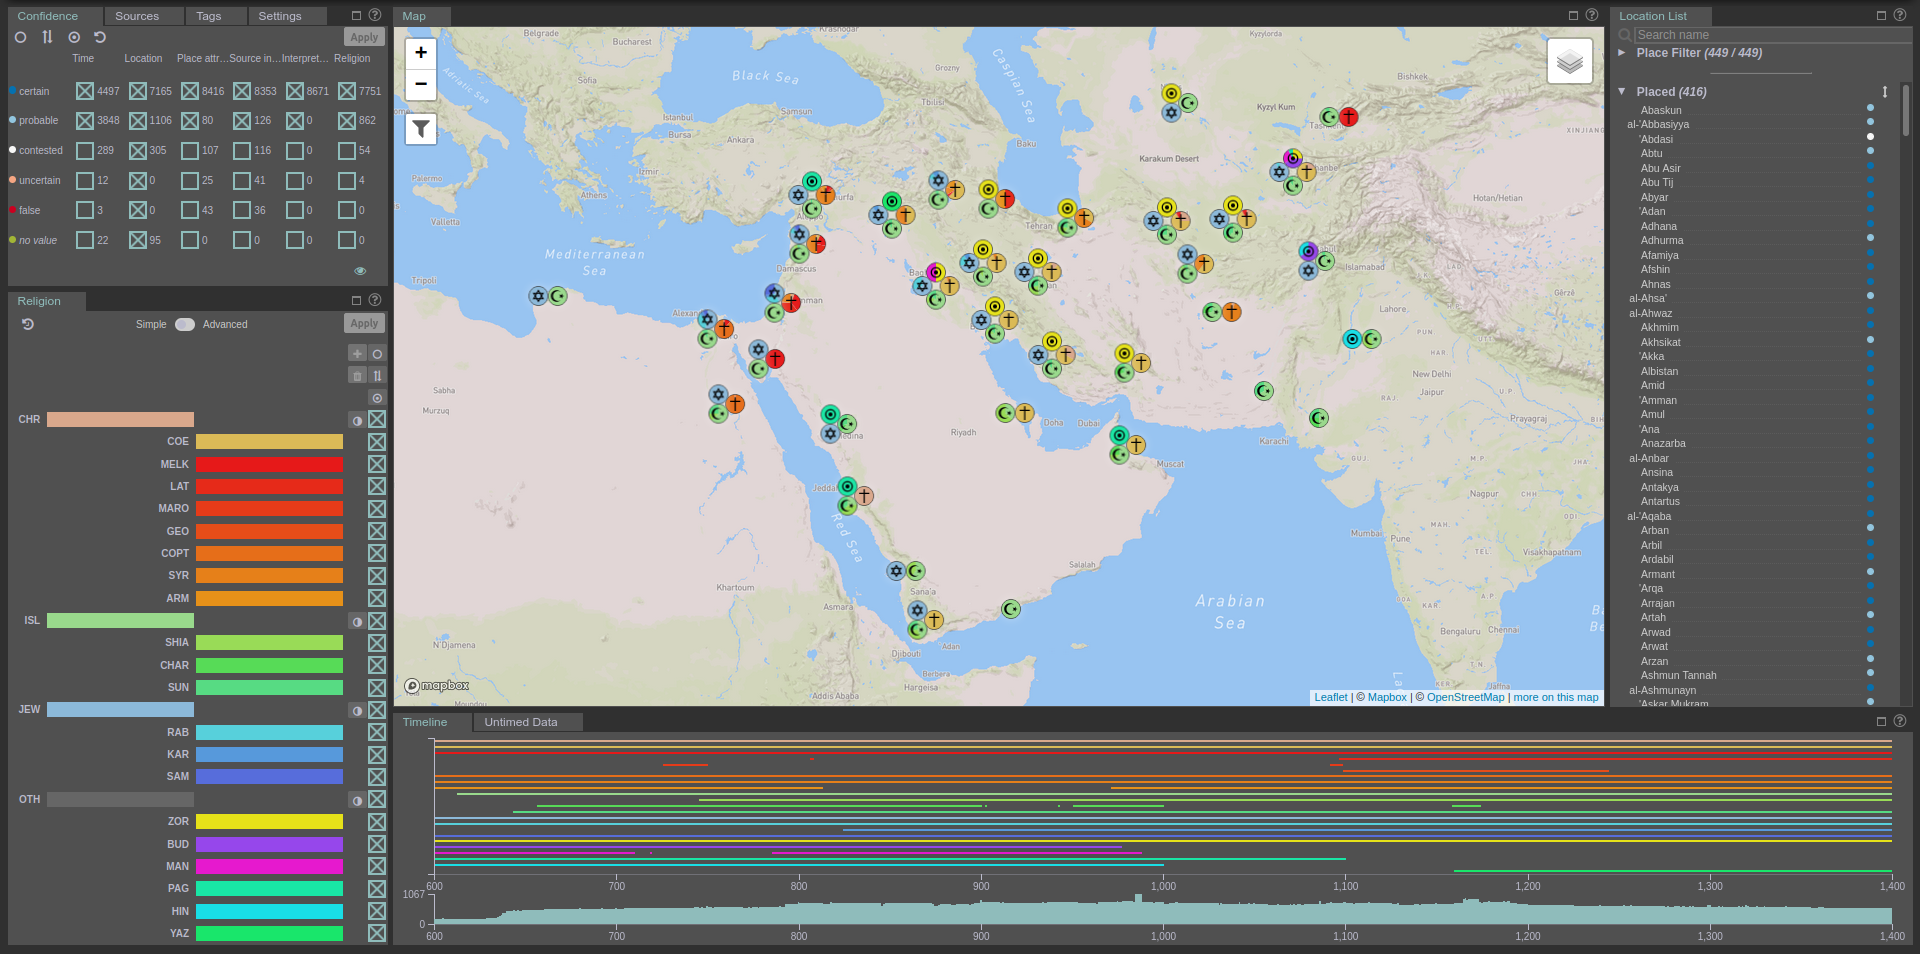
\includegraphics[width=\textwidth]{../src/assets/visualization-documentation/full-vis-screenshot.png}
  \caption{
    Screenshot of the visualization, consisting of multiple coordinated views.
    Each view visualizes one aspect of the data, and interactions with one view are reflected in the others.
  }
  \label{fig:full-vis-screenshot}
\end{figure}

A multiple coordinated views (MCV) visualization consists, as the name implies, of multiple \emph{views.}
These views are visually separated, either just by empty space between them or by borders.
In \textsc{Damast} (see \cref{fig:full-vis-screenshot}), each view is displayed in a separate user interface (UI) element.
These UI elements are called \emph{panes} and can be resized, rearranged, or maximized, similar to the way windows can be interacted with in an operating system such as Microsoft Windows.

In an MCV visualization, each view shows a \emph{different perspective} on the \emph{same data;}
that is, the view visualizes a specific aspect of the data.
In \textsc{Damast}, one view visualizes the temporal aspect of the data (the timeline), another view the geospatial aspect (the map), and so on.
However, the same underlying data (pieces of evidence) is shown in each view.
Further, the views are \emph{coordinated,} meaning that interaction with one of the views is reflected by changes in other views.
\Cref{fig:full-vis-screenshot} provides an example:
Filtering by time range in the timeline view also affects the data shown in the map view.
After filtering, only places with evidence from that time range are shown.
For more details on the different interactions; see \cref{sec:terminology-filtering,sec:terminology-selection,sec:terminology-brushing-linking}.


\subsection{Filtering}
\label{sec:terminology-filtering}

\textsc{Damast} is a \emph{top-down visualization,} meaning that initially, all data is shown, and users can then \emph{drill down} into that data to find smaller, more specific subsets of the data.
The drill-down is realized by applying \emph{filters} to the data.
A filter decides for each datum whether it matches specific criteria or not.
Applying a filter to a dataset results in a subset of the dataset (not necessarily a \emph{proper subset} in mathematical terms).

An example for a filter in \textsc{Damast} is to select a time span from the timeline.
The filter then specifies the time span within which the evidence must lie to still be visualized.
Another example is to specify one or more sources that the evidence must be attributed to;
in this case, the data visualized stems from these sources only.

Our MCV visualization (\cref{sec:terminology-mcv}) implements \emph{multi-faceted filtering.}
That means that each view can have a separate filter active at the same time.
Because the views show different aspects of the same data, the filters, too, apply to different aspects of the data:
The timeline filter applies to the temporal aspect of the evidence, the map filter applies to the geospatial aspect of the evidence, and so on.

Generally, one should be aware of how these filters work \emph{between} as opposed to \emph{within} views.
\emph{Between views,} the filters are applied in conjuction;
that is, a piece of evidence is shown only if it matches \emph{all} filters.
For example, if the map and timeline both have an active filter, evidence is only visualized if it is within the specified time span \emph{and} within the specified geographical region.

\emph{Within views,} the filters are applied in disjunction; that is, a piece of evidence matches the filter if it matches \emph{any} of the criteria.
For example, if a religion filter with two religions is active, it matches evidence that has \emph{either} one \emph{or} the other religion.
This behavior is logical, in that there can be no evidence that has \emph{both} religions at the same time, or is attributed to two places at once.

\subsection{Selection}
\label{sec:terminology-selection}

\emph{Selection} is a user interaction with the data.
In \textsc{Damast}, selection is done by \emph{clicking} on some visual element with the computer mouse.
For example, clicking a glyph (i.e., a symbol representing one or more places) in the map informs the visualization that the user selected that glyph.
Note that what the visualization does \emph{in reaction to} clicking is no longer part of the selection itself.
For the main purpose of selection, see \cref{sec:terminology-brushing-linking}.

\subsubsection{Brushing and Linking}
\label{sec:terminology-brushing-linking}

\begin{figure}[tb]
  \centering
  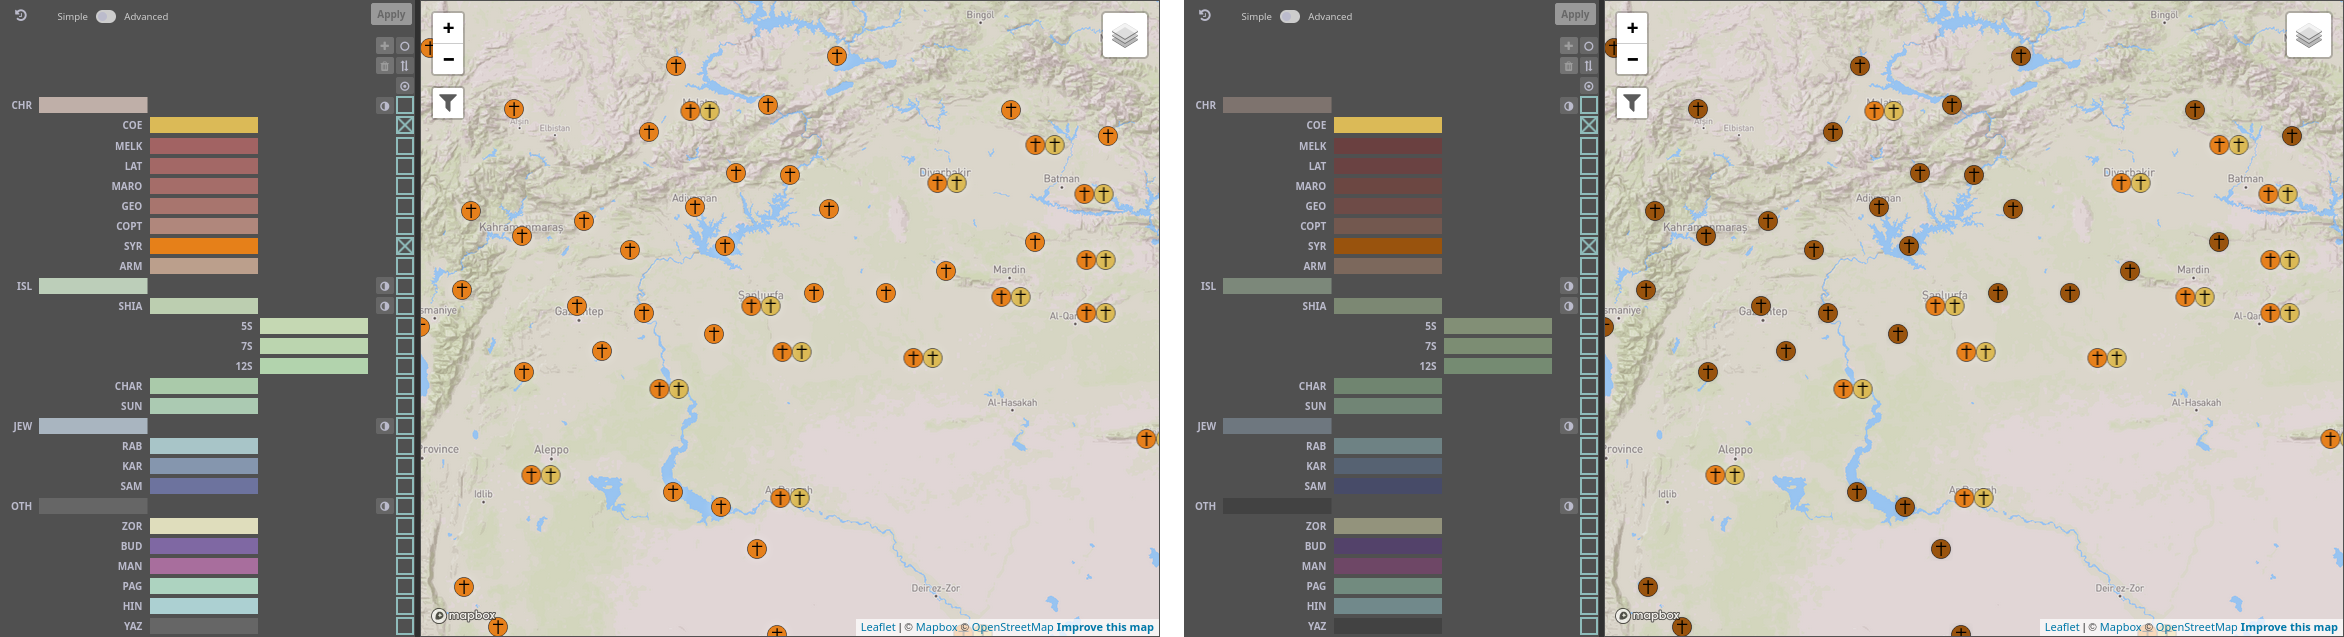
\includegraphics[width=\textwidth]{../src/assets/visualization-documentation/brushing-linking-horizontal.png}
  \caption{
    Example for brushing and linking.
    Evidence of two religious groups is visualized (left).
    After selecting the Church of the East (COE) in the religion view, evidence of COE is \emph{brushed,} and the respective visual representations of that data are \emph{linked} in all views (right).
    In the religion view, all other religions' representations are desaturated and darkened.
    In the map, all map glyphs for places or clusters of places not containing COE evidence are darkened and desaturated.
  }
  \label{fig:brushing-linking}
\end{figure}


\emph{Brushing and linking} is a process used in interactive MCV visualizations to help users understand the connection between different views, or rather, between different aspects of the visualized data.
First, the user selects (\cref{sec:terminology-selection}) some visual element in the visualization.
The visualization interprets that selection, and performs \emph{brushing} on the underlying data that is represented by that element.
Next, the visualization \emph{links} the brushed data in \emph{all views} by applying specific highlighting to them.

In \textsc{Damast}, brushing always happens on a subset of the visualized evidence.
The linking is then done in all views, including the one the selection and brushing originated from.
In most views, we display linked elements by keeping their saturation, while all elements that are \emph{not} linked are desaturated and darkened.
A notable exception to this behavior is the timeline, where linking will show the temporal data from the brushed subset only, while all other data will be hidden.

Clicking on the same selected element again will \emph{revert} the selection and also clear the brushing and linking.
Selecting any other visual element will instead \emph{replace} the selection and brushing and linking will apply to the new subset accordingly.
In the map, the brushing and linking can also be cleared by clicking in an empty place.

A source of confusion with the term \emph{\enquote{brushing}} can be that it is interpreted in the sense of \enquote{paint brush;}
in that sense, the brushing itself would be a change of the visual representation of the elements (e.g., their being highlighted).
However, this change of the visual representation is the \emph{linking} part.
Rather, \emph{brushing} should be understood as in \emph{touching (or brushing) with one's fingers}:
\emph{Selecting} a subset of data touches (brushes) them, and the subset of data is highlighted in all views, thereby visually \emph{linking} the data to the selection and providing context.

\Cref{fig:brushing-linking} shows an example of brushing and linking in \textsc{Damast}:
Evidence from two religions is visualized.
Clicking on one of these religions in the religion view \emph{selects} it and \emph{brushes} the respective evidence.
The visual representations of this subset of evidence is then \emph{linked} in all views by desaturating the elements that are not part of the subset.


\subsection{Visualization Types}

A number of visualization types are used in \textsc{Damast}.
The proper scientific terms are used in the description below, and are introduced here.

\subsubsection{Bar Chart and Stacked Bar Chart}

In a \textbf{bar chart,} categories are represented by rectangular bars, usually with a common baseline in one dimension, and a common width.
The height of each bar encodes a value associated with the respective category.
Bar charts can be horizontal as well, in which case the height of the bars is constant, and the width encodes value instead.
In \textsc{Damast}, the bar charts used are horizontal, for example in the source view (\cref{sec:source}).

A special case of bar charts are \textbf{stacked bar charts,} in which each category, or bar, is further divided.
Each segment of the bar encodes a sub-category's value.
In \textsc{Damast}, stacked bar charts are used in the untimed data view (\cref{sec:untimed-data}), where each general religious affiliation is represented by a bar, and its specific religious groups by segments of that bar.
In \emph{all data mode,} all regular bar charts turn into stacked bar charts, with one segment for active data, and one for filtered-out data.
Similarly, in \emph{confidence mode,} a segment for each represented level of confidence is shown.

An even more special case is the \textbf{normalized} stacked bar chart, where the width (or height) of the bars is constant across bars as well.
Hence, the width of individual segments encodes their \emph{relative} proportion within the parent category.
Normalized stacked bar charts appear in the source view (\cref{sec:source}), where they show the distribution of religious groups (or confidence levels) within each source.

\subsubsection{Stacked Area Chart}

An \textbf{area chart} shows changes of one value in dependence of another value, usually time.
It is similar to a line chart, but the area between the line and the \emph{x}-axis is filled in.
A \textbf{stacked} area chart, similar to a \emph{stacked bar chart,} is a chart where multiple such areas are stacked on top of each other.
This representation makes it harder to read individual values, but provides a better understanding of the sum over all categories and general trends.
In \textsc{Damast}, stacked area charts are used in the \emph{quantitative mode} of the timeline (\cref{sec:timeline}).

\subsubsection{Indented Tree}

An \textbf{indented tree} is a visualization for hierarchies.
Nodes of the hierarchy are represented as elements placed in individual rows, or columns.
To signify parent-child relationships, children are \emph{indented} further than their parents.
Indented trees are often used in file managers to show directory structures, or in mail programs to display e-mail threads.
In \textsc{Damast}, an indented tree visualization is used to show the religion hierarchy (\cref{sec:religion-hierarchy}).

\subsubsection{Gantt Chart}

A \textbf{Gantt chart} is a visualization for \emph{time spans.}
Each time span is visualized by a rectangle, where the position of the left and the right side of the rectangle signify the start and end of the span.
The rectangle heights are usually fixed, and the vertical position can be used to signify categories, or dependencies.
Gantt charts are often used to visualize dependent periods in project planning.
In \textsc{Damast}, Gantt charts are used in the \emph{qualitative mode} of the timeline (\cref{sec:timeline}).


\section{Visualization}

This section provides documentation on the different parts of the \emph{visualization,} what they show, and how they can be interacted with.
The individual \emph{views} and their respective functionalities are explained.
These explanations can also be accessed individually from within the visualization by clicking on the
\tikz\node[circle,draw,inner sep=0.1pt]{\scriptsize?};
question mark icon in the upper right corner of each view.


\subsection{Settings Pane}
\label{sec:settings-pane}

\begin{figure}[tb]
  \centering
  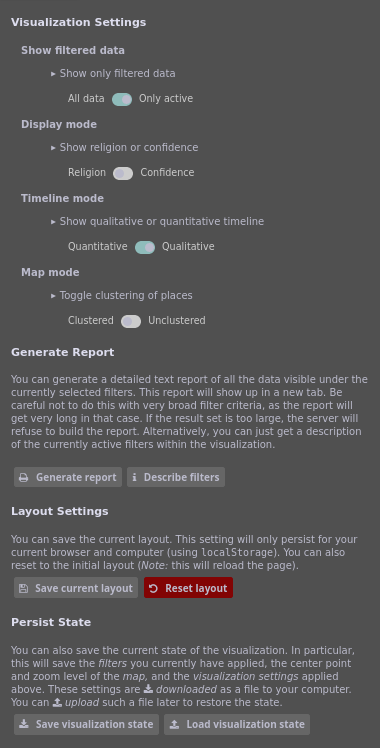
\includegraphics[width=0.3\textwidth]{../src/assets/visualization-documentation/settings.png}
  \caption{
    The settings pane.
  }
  \label{fig:settings}
\end{figure}

This pane shows different \textbf{settings} pertaining to the visualization.
It also offers some \textbf{functionalities} to store or load these settings and to generate reports from the currently shown data.


\subsubsection{Visualization Settings}
\label{sec:settings-vis-settings}

These are settings that directly affect the visualization.
In particular, they control which data is shown and in which way.

\subsubsection{Show filtered data}
\label{sec:settings-all-data-only-active}

This switch controls if data is visualized although it \textbf{does not match the currently applied filters.}
If \emph{All data} is selected, non-matched data is shown in less saturated colors.
Otherwise, it is not shown at all.


\subsubsection{Display mode}
\label{sec:settings-display-mode}

This switch controls \textbf{which aspect of the data} is mapped to color.
If \emph{Religion} is selected, religion is used for coloring, using the color scheme in the \emph{religion view.}.
If \emph{Confidence} is selected, the level of confidence is used, using the color scheme in the \emph{confidence view.}
The \emph{aspect of confidence} used for the visualization can be selected in the \emph{confidence view;}
there, the currently used aspect is indicated with an eye symbol below the column.


\subsubsection{Timeline mode}
\label{sec:settings-timeline-mode}

This switch controls whether the \emph{timeline} shows \textbf{a qualitative summary or quantitative information}.
If \emph{Quantitative} is selected, the number of pieces of evidence of that type in that year is represented by the height of the area.
The \emph{timeline} then looks like a \emph{stacked area chart.}
If \emph{Qualitative} is selected, the \emph{timeline} only shows \emph{whether} there are pieces of evidence of that type each year.
The \emph{timeline} then looks like a \emph{Gantt chart.}


\subsubsection{Map mode}
\label{sec:settings-map-mode}

This switch controls whether map glyphs are \textbf{\emph{clustered} or \emph{unclustered.}}
By default, glyphs are \emph{clustered:}
zooming out will lead to religions attributed to different places being \emph{clustered} (\enquote{summarized}).
(Note that for these clusters, all places are treated equally;
for example, the distribution of religions of place A and place B is combined without taking into account any further aspects of A or B.)

If glyphs are \emph{unclustered,} one small symbol per place and religion is shown.
\emph{Note:} This mode may lead to overlap of symbols when zooming out even to a relative small scale and should, thus, be used with due caution when interpreting the results.


\subsection{Generate Report}
\label{sec:generate-report}

With this feature, a detailed \textbf{text report} can be generated, which presents all data matched by the currently applied filters.
The report will also contain information on the filter criteria that led to the selection of data.
After clicking \emph{Generate report,} a new tab in the browser will open.
A report can also be created by uploading a \emph{visualization state} that was saved and downloaded beforehand (\cref{sec:settings-persist-state}).

\emph{Note:} It is not advised to create a report with very broad filter criteria, as it will become very long and thus difficult to handle.

This section also has a button labeled \emph{Describe filters.}
Clicking this button will open a small window (a so-called modal window) that describes the currently active filters in text form.
This description is the same as the one at the top of a report.


\subsection{Layout Settings}

The \textbf{current layout} of the visualization; i.e., the arrangement of the views, can be saved.
This feature is only available if the option \emph{All cookies} is accepted in the \emph{Cookie preferences} (accessible through the menu bar on top).
The \emph{layout settings} will only persist for the currently used browser and computer (using \verb!localStorage!).
You can also reset the layout to the initial state. Note that this will reload the page.

\emph{Note:} Depending on your browser settings, cookies may be deleted after closing the browser, which leads to the loss of the saved \emph{layout settings.}


\subsubsection{Persist State}
\label{sec:settings-persist-state}
\label{sec:vis-reproducible}

With this feature, the current \textbf{overall state} of the visualization can be saved.
In particular, this will save

\begin{itemize}
  \item the \emph{filters} that are currently applied,
  \item the center point, zoom level, and visible layers of the \emph{map,} and
  \item the \emph{visualization settings} (\cref{sec:settings-vis-settings}).
\end{itemize}

These settings are \emph{downloaded} as a file to the computer.
Later, such a file can be \emph{uploaded} to restore the state.
The file can also be shared to either present your results or to (re-)generate a report based on the filters.


\subsection{Map}
\label{sec:map}

\begin{figure}[tb]
  \centering
  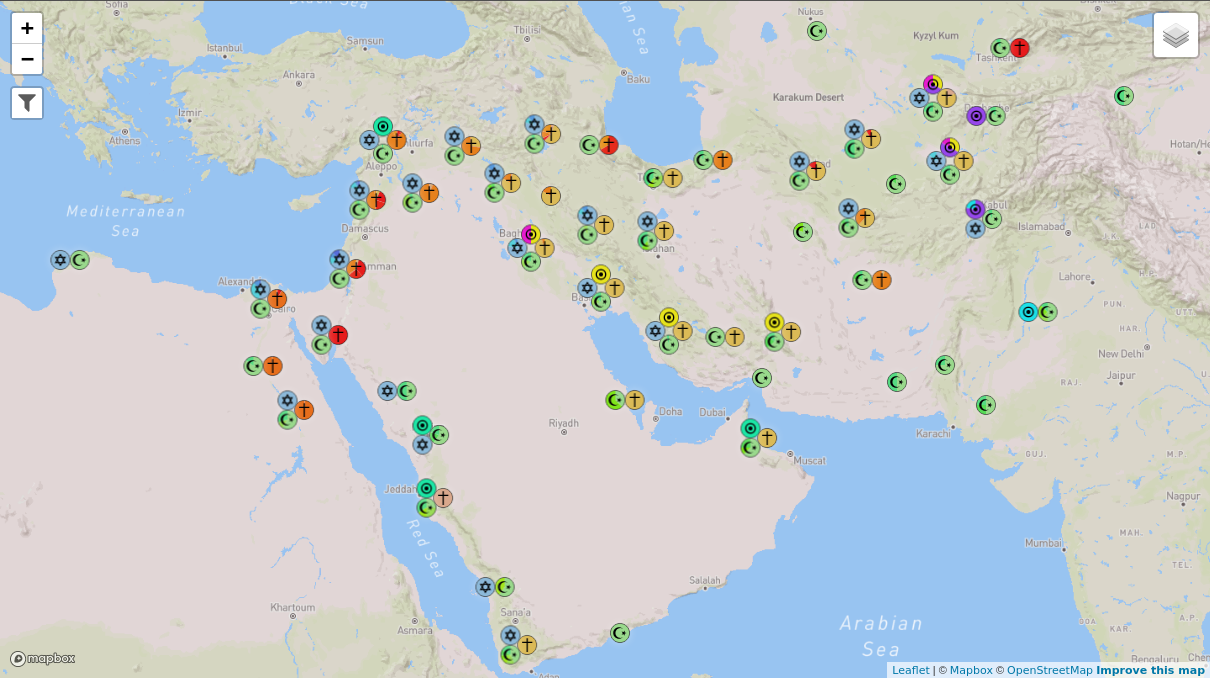
\includegraphics[height=5cm]{../src/assets/visualization-documentation/map-1.png}%
  \hfill%
  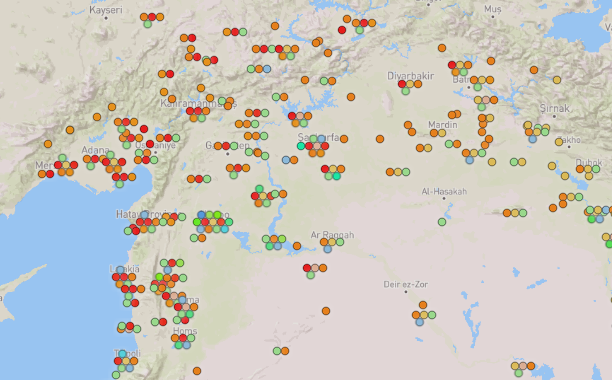
\includegraphics[height=5cm]{../src/assets/visualization-documentation/map-2.png}
  \caption{
    The map pane in \emph{clustered} (left) and \emph{unclustered} (right) \emph{map mode.}
  }
  \customlabel{fig:map-1}{ left}
  \customlabel{fig:map-2}{ right}
\end{figure}

The \textbf{\emph{map}} visualizes the geographical aspect of the data, i.e., evidence for the presence of religious groups at different locations.


\subsubsection{Content}

\paragraph{Map Glyphs.}
Pieces of evidence are represented by so-called map glyphs.
By default, these map glyphs are \textbf{clustered} (i.e., \textbf{aggregated,} or \enquote{summarized}).

This aggregation depends on the data currently active and on the current zoom level of the map;
that is, once the zoom level or filters are changed, the map is populated with glyphs according to the aggregation rules;
simply \emph{panning} the map will not affect the map glyphs.
More details are given below.

This \emph{map mode} is called \emph{clustered.}
It can be changed in the settings (\cref{sec:map-unclustered-mode,sec:settings-map-mode}).


\subparagraph{Aggregation of Locations.}
Locations are \emph{aggregated} to eliminate overlap, and so, by default, each map glyph represents \textbf{one or more} cities, depending on the zoom level.
\emph{Note:} For this aggregation, all places are treated equally;
that is, the distribution of religions of place A and place B is combined without taking into account any further aspects of A or B.

When \emph{hovering} over a glyph, it loses opacity and the aggregated locations are indicated on the map as small turquoise dots (maybe partially covered by the glyph).
While hovering, a tooltip is also shown, which provides information on the number of pieces of evidence, of religions, and of places related to the glyph.
As long as the glyph does not aggregate more than five places, the toponym, geographical coordinates, and more information on the pieces of evidence belonging to that place are provided for each place.
Even more details are provided if the glyph only represents one place.

\subparagraph{Aggregation of Religions.}
A map glyph consists of up to four circles, each representing a general religious affiliation with a distinct symbol and color:

\begin{itemize}
  \item Christianity: cross, red/orange
  \item Islam: crescent, green
  \item Judaism: Star of David, blue
  \item Other: dot, varying colors
\end{itemize}

Generally, multiple religious groups belonging to the same general religious affiliation are aggregated to one circle.
This circle then functions like a pie chart:
in \emph{religion mode} (set by default), each piece of the pie chart represents a different religious group in its respective color and the piece's size shows the amount of pieces of evidence of that religious group relative to the overall evidence of its general religious affiliation.
In \emph{confidence mode,} the division of the circle or pie chart is based on the pieces of evidence attributed with different levels of confidence and is colored accordingly.

However, if, regarding \emph{all} map glyphs currently displayed, no more than four religous groups are to be represented, there can be more than one circle representing a general religious affiliation.
For instance, if only COE (Church of the East), SYR (Syriac Orthodox Church), and SUN (Sunni Islam) are filtered using the \emph{religion view,} any given map glyph cannot have more than three circles.
Accordingly, both COE and SYR will be represented by an individual circle with a cross and the respective color.
Note that this aggregation may result from other filters or interactions with the map, not just filtering using the \emph{religion view,} as the map glyphs are dynamically altered based on many different criteria.

Note that placement and aggregation of map glyphs depends on the data currently active as well as the zoom level---not, however, on the current center of the map.
In other words, \enquote{all map glyphs \emph{currently displayed}} include map glyphs outside the current scope of the map that will appear when panning the map.

If in at least one glyph currently displayed multiple religious groups are aggregated into one circle, this same aggregation will apply to \emph{all} other glyphs as well, even if, in sum, they have less than four circles and would not be aggregated.
Otherwise, the perceived variety and distribution of religions would be skewed;
for example, a location with only two Christian groups would be represented by a map glyph with two circles for Christianity, while a location with many Christian groups as well as other groups would be displayed with only one such circle.

In \emph{only active} mode, data that has been filtered out disappears from the map.
Note that this can lead to glyphs having less circles, if, for example, all Christian data of a glyph has been filtered out.
In \emph{all data} mode, data that has been filtered out is indicated by less saturated colors.

\paragraph{Unclustered Mode.}
\label{sec:map-unclustered-mode}
The aggregation or clustering of places can be turned off in the \emph{settings pane.}
In this \emph{map mode,} called \emph{unclustered,} each location is represented by an individual glyph.
Here, the glyphs consist of smaller circles, one for each religious group.
These circles are arranged in a hexagonal pattern.
Overlap can and will happen in this mode, even when zooming out to a relative small scale.
\emph{Z}-ordering of the glyphs ensures that glyphs with fewer religious groups appear in front of larger glyphs with more religious groups.

\emph{Note:} For both modes, the specific way of representing the data should be considered when interpreting the results.


\paragraph{Layers.}
The map provides multiple layers, which can be controlled from the layer control in the upper right corner.
One of two \emph{base layers} is always selected and shown:
by default, a layer based on a custom map from MapBox\footnote{\url{https://www.mapbox.com/about/maps}} is selected, which shows topological features but no geo-political borders (i.e., borders of modern nation states).
As an alternative, a map provided by the Digital Atlas of the Roman Empire\footnote{\url{https://imperium.ahlfeldt.se/}} (DARE) can be selected as the base layer.

In addition, one or more overlay layers can be shown:

\begin{description}
  \item[Markers]
    consists of the clustered or unclustered map glyphs. It is shown by default.
  \item[Diversity Markers]
    displays all locations, without clustering, each colored according to its religious diversity (i.e., the number of distinct religions present in each place). The color scale Viridis\footnote{\url{https://github.com/d3/d3-scale-chromatic\#interpolateViridis}} is used, where low values are mapped to violet, and high values to yellow.
  \item[Diversity Distribution]
    shows an estimation of the religious diversity and is colored according to the same scale as the \emph{diversity markers.}
  \item[Distribution]
    shows an estimation of the density of pieces of evidence.
\end{description}

\emph{Note:} The two layers for diversity (one displaying markers, the other displaying a heatmap) are \emph{alternative} representations of the \emph{same} data.
Thus, they should not be both displayed at the same time.
Similarly, the two layers using markers (the default one displaying map glyphs and the one displaying markers of diversity) should not be shown together.


\paragraph{What the Map is \emph{not} Showing.}
\textsc{Damast} visualizes religious constellations in cities and towns of the Islamicate world with static Non-Muslim communities.
The map does \emph{not} depict a representation of the population density in the medieval Middle East.
In other words, an area with no or only few map glyphs is not necesarrily less populated than other areas.
The map makes no claim to be complete, nor does it show the general distribution of religions in a given area.

Empty areas on the map can have multiple reasons:

\begin{itemize}
  \item The area is outside the geographical scope of \textsc{Damast}, e.g., Europe.
  \item No data for a city was collected.
  \item No data on non-Muslim communities was available.
\end{itemize}

Furthermore, in \emph{clustered} mode, the overall size of the map glyphs (i.e., the number of circles) does \emph{not} directly correlate with the number of religions or pieces of evidence;
for instance, a map glyph with three circles does not necessarily represent more pieces of evidence than one with only two circles.


\subsubsection{Interaction}

The map can be interactively zoomed and panned (i.e., the center of the map is moved).

\paragraph{Selection.}
Clicking on a map glyph will \emph{select} the represented places, \emph{brush} the represented data, and \emph{link} the respective data in the rest of the views.
Likewise, brushing data in other views will link the respective places in the map.
Also, selecting a place in the location list will pan the map to center on that place.
Map glyphs that are not linked will be displayed in less saturated colors.
Linking persists when zooming, even if clustered glyphs split up or merge.
Note, however, that a map glyph often represents more than one location.
In this case, \emph{all} of the circles belonging to the glyph are highlighted, even if the linking only refers to part of the evidence.
For instance, a place from the \emph{location list,} which only has pieces of evidence of the general religious affiliation \enquote{Christian}, may be selected.
If this place is aggregated with other places that additionally have, for instance, Islamic pieces of evidence, both the circle with the crescent as well as the one with the cross are highlighted.

\begin{figure}[tb]
  \centering
  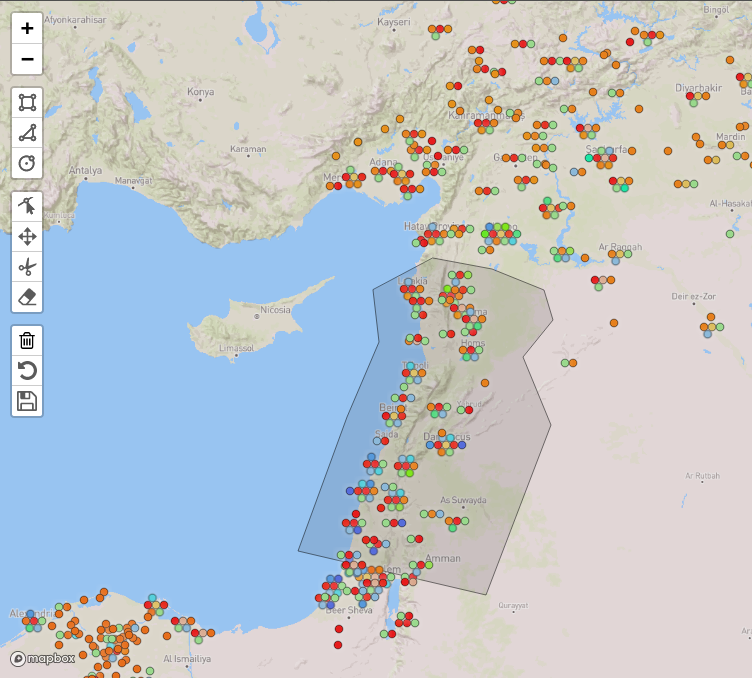
\includegraphics[width=0.5\textwidth]{../src/assets/visualization-documentation/map-3.png}
  \caption{
    The map pane with the Geoman editor open, and a polygon being edited.
  }
  \label{fig:map-3}
\end{figure}

\paragraph{Geographical Filtering.}
Evidence can be filtered by geographical location.
This is done by drawing the respective bounding shapes into the map.
For this, the Leaflet plugin for Geoman\footnote{\url{https://geoman.io/leaflet-geoman}} is used.
The respective tools to control the filters are available by clicking on the button with the funnel in the upper left corner of the map, below the zoom buttons.
The button then expands to a set of controls, arranged in three blocks:
the first block for adding elements, the second for editing them, and the third to apply, remove or revert the filters.
These are described in detail below.
Tooltips are shown when hovering over the individual buttons.

The first block is for \emph{adding} new elements to the bounds:
\begin{itemize}
  \item A rectangular area can be added, by first clicking in the map to select one corner, then moving the mouse, and clicking again to select the opposite corner.
  \item
    The second option is to add a polygon.
    Here, a new point is appended to the polygon each time you click in the map.
    To complete the polygon, click on the first node.
  \item
    The last option is to add a circle.
    Click once to select the center, move the mouse, then click again once the circle has the appropriate radius.
    Note that the circle is converted to a GeoJSON polygon when saving.
\end{itemize}

The second block contains controls for \emph{editing} existing elements.
It is possible to
\begin{itemize}
  \item move points on existing shapes,
  \item move entire shapes,
  \item cut (subtract) a polygon from an existing shape, and
  \item remove entire shapes.
\end{itemize}
Note that polygons can only be moved or removed individually \emph{before} they have been applied as filters.

The last block contains controls to \emph{apply} the created bounds to the dataset filter:

\begin{itemize}
  \item The trash can button removes all existing shapes.
  \item The  undo button reverts the bounds back to the state of the currently active filter, i.e., the geographical filters applied last.
    It then collapses the menu.
  \item The save button applies the new bounds to the dataset filter, and then closes the editor.
\end{itemize}


\subsection{Location List}
\label{sec:location-list}

\begin{figure}[tb]
  \centering
  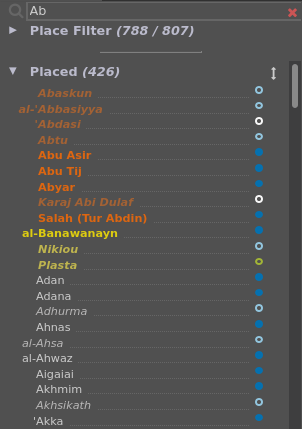
\includegraphics[width=0.25\textwidth]{../src/assets/visualization-documentation/location-list-1.png}
  \caption{
    The location list.
    The \emph{confidence of location} is indicated by a colored marker behind the place name.
    Places that match the search term at the top are highlighted in orange if their primary name matches, or in yellow if an alternative name matches.
    Names are shown in italics, darker, and desaturated if their level regarding confidence of location is not currently checked.
  }
  \label{fig:location-list-1}
\end{figure}

In this view, \textbf{all locations} in the data are listed, using their \emph{main toponym} as place name.
Places can be searched, selected and filtered.


\subsubsection{Contents}
\label{sec:location-list-contents}

The view consists of several sections:

\begin{itemize}
  \item a \emph{search} field;
  \item a \emph{place filter;} and
  \item the actual \emph{location list,} consisting of two lists, \emph{Placed} and \emph{Unplaced,} representing locations with and without geo-coordinates, respectively.
\end{itemize}

Detailed descriptions how to use the \emph{search} field and the \emph{place filter} are found below under \emph{\enquote{Interaction}} (\cref{sec:location-list-interaction}).
In what follows, the two lists are described.

\label{sec:location-list-unplaced}
The list \emph{Placed} contains all locations for which a geographical position is known.
The list \emph{Unplaced} contains all locations for which a geographical position is not (yet) known;
in this case, the \emph{confidence of location} is attributed with \emph{no value} and colored accordingly.

\emph{Note:} Missing data is normal during research and while entering data is still in progress.
However, missing data can severely affect confidence in the visualization if not properly communicated.
We have therefore chosen to make missing geographical locations and time information explicit in separate views of this interface (apart from the section \emph{Unplaced} in the \emph{location list,} see the untimed data view (\cref{sec:untimed-data}).
This also allows for searches directed at data in need of improvement.

The position of the two lists can be swapped by clicking on the swap button.
The following is true for both lists:
Each line in the lists represents one location.
Locations are listed using their \emph{main toponym} as place name.
Accordingly, looking through the lists with a specific place name in mind, if this place name is not the \emph{main toponym,} the location is not found and should be searched in the \emph{Search field.}
There, \emph{alternative names} are considered as well (\cref{sec:location-list-search-toponyms}).

The place names are sorted alphabetically, disregarding a prefix of apostrophes (e.g., for the letter \emph{'ain}) or Arabic definite articles;
for instance, \enquote{Amid} comes before \enquote{'Amman}, and \enquote{Jubayl} comes before \enquote{al-Juma}.
In \emph{only active} mode (\cref{sec:settings-all-data-only-active}), only places with pieces of evidence matching the current filters are listed.
When \emph{hovering} over the line with the mouse, a \emph{tooltip} (\cref{fig:location-list-2}) with additional information is shown, that is:

\begin{itemize}
  \item place type,
  \item geographical location (i.e., coordinates),
  \item confidence of location,
  \item alternative names,
  \item external URIs referencing the same place.
\end{itemize}

Also, while hovering, a link symbol appears at the very end of the line (\cref{fig:location-list-2}).
Clicking the symbol opens an overview for this place, the so-called \emph{place URI page} (\cref{sec:place-uri-page}).
\emph{Note:} If the user has rights to edit the database, clicking the symbol leads to the respective entry of the location in the database instead.

Behind the place name, the \emph{confidence of location} of each place is shown as a small, colored circle.
The color scale is the same as in the \emph{confidence view.}
In \emph{all data} mode (\cref{sec:settings-all-data-only-active}), when the filter set for \emph{confidence of location} does not match the place’s confidence of location, this confidence circle is not filled.
Also, the name is displayed in italics, darker, and in less saturated colors in that case.

\begin{figure}[tb]
  \centering
  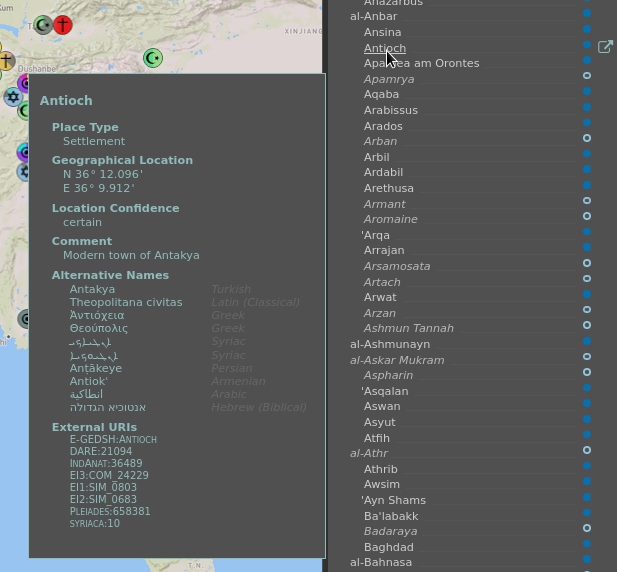
\includegraphics[width=0.5\textwidth]{../src/assets/visualization-documentation/location-list-2.png}
  \caption{
    A tooltip in the location list, for the place Antioch.
  }
  \label{fig:location-list-2}
\end{figure}


\subsubsection{Interaction}
\label{sec:location-list-interaction}

\paragraph{Selection.}
Individual locations can be selected by clicking on the respective line of the list.
This will highlight the location, bring it to the top of the list and show a short vertical line to the left of the place name.
Data related to the selected location will be \emph{linked} in all other views, while non-selected data will be displayed in less-saturated colors.

\paragraph{Searching for Toponyms.}
\label{sec:location-list-search-toponyms}
It is possible to \textbf{search for a specific place using different toponyms} in the search field at the top.
Non-Latin scripts can be used for searching, too.
Typing a search query in that field will highlight the search results in bold orange and sort them to the top of the list.
The search matches not only the \emph{main toponym} but also \emph{alternative names;}
for example, \enquote{Edessa} will find the respective place under its \emph{main toponym} \enquote{al-Ruha}.
Matches to \emph{alternative names} that do not match the \emph{main toponym} are sorted after \emph{main toponym} matches and highlighted in bold yellow.

Apart from toponyms, \textbf{external URIs} can be entered in the \emph{search field.}
For example, \verb!syriaca:10! or \verb!syriaca.org/place/10! finds Antioch.
The search is partially case-sensitive:
\verb!ask! finds both \enquote{Daskara} as well as \enquote{al-Askar Mukram}, while \verb!Ask! only finds \enquote{al-Askar Mukram}.
The search field additionally supports JavaScript-style \textbf{regular expressions.}
For example, searching for \verb!Bagh?dad! would find \enquote{Bagdad} as well as \enquote{Baghdad}, because \verb!h! followed by \verb!?! matches no \enquote{h} or exactly one \enquote{h}.
For further reference, refer to the MDN documentation\footnote{\url{https://developer.mozilla.org/en-US/docs/Web/JavaScript/Guide/Regular_Expressions}}.

\paragraph{Filtering.}
The expandable section \emph{Place Filter} at the top of the view allows to \textbf{filter evidence by place.}
When expanded, a list of all places in the database is shown.
If, however, something has been entered into the \emph{search field,} only places matching the search are listed.

This list is used to include or exclude places from the so-called \emph{place set,}
that is, the set of places currently active.
For instance, if Baghdad is excluded from the \emph{place set,} all pieces of evidence attributed to Baghdad are filtered out.
Keep in mind that, when \emph{all data} mode is active, pieces of evidence attributed to places excluded from the \emph{place set} are visible but displayed in less saturated colors.

A place can be removed from the place set by clicking on the \emph{red minus} on its right, or added to the place set by clicking on the \emph{green plus.}
Note that the selection is not applied until the \emph{Apply} button is clicked.
This button is disabled if the selected filters are matching the data currently visualized.

A symbol to the left of the place name indicates the current state of the place:

\begin{itemize}
  \item a turquoise check mark if the place is in the currently active \emph{place set;}
  \item no mark if the place is not in the currently active \emph{place set;}
  \item a grey cross if it will be excluded from a new \emph{place set} which has not been applied yet; and
  \item a green check mark if it will be added to a \emph{new place} set which has not been applied yet.
\end{itemize}

\textbf{Place sets can be saved} using the \emph{Save} button under the list.
For users with access to the database, this will store a place set in the database under the name entered by the user.
For users without access to the database, the place set will only be saved to \verb!localStorage!.
This feature is only available if the option \emph{all cookies} is accepted in the \emph{cookie preferences} (accessible through the menu bar on top).
By clicking the \emph{Load} button, a saved \emph{place set} can be loaded back into the filter.
\emph{Note:}: Depending on your browser settings, cookies may be deleted after closing the browser, which leads to the loss of the saved \emph{place sets.}

\paragraph{Buttons Facilitating Creating \emph{Place Sets}.}
Buttons in the top left corner help in editing the \emph{place set} on a larger scale:

\begin{description}
  \item[The revert button]
    will \emph{revert} the changes to the \emph{place set;}
    that is, the \emph{place set} will match the current filters. \\
    \emph{Note:} Because of the functionalities detailed below, the \emph{place set} will \textbf{not} update from the database when other filters change;
    it changes only with the initial load and loads of the visualization state (\cref{sec:settings-persist-state}).
    Instead, resetting the \emph{place set} is left to the user, which allows to build up a place set incrementally as illustrated by the example below.

  \item[The empty circle button]
    will \emph{uncheck} all places;
    that is, no place would be included in the intended \emph{place set} after application.
  \item[The exchange button]
    will \emph{invert} the current marks;
    that is, all places that were marked are unmarked, and vice versa.
  \item[The circle button with dot inside]
    will \emph{check} all places;
    that is, all places would be included in the intended \emph{place set} after application.
  \item[The set union button]
    will \emph{extend} the \emph{place set} (PS) by all places currently shown in the \emph{location list} (LL) (\cref{sec:location-list-contents}).
    That is, all places that were in the \emph{place set} before are still there, and \emph{additionally} all places from the \emph{location list} are checked.
    The result is the \emph{set union} of the previous \emph{place set} and the current \emph{location list:}

    \[ \text{PS}_\text{new} = \text{PS}_\text{old} \cup \text{LL} \]
  \item[The set intersection button]
    will \emph{restrict} the \emph{place set} to contain only a subset of its current contents, namely those places that are \emph{also} in the \emph{location list.}
    The result is the \emph{set intersection} of the \emph{place set} set and the current \emph{location list:}

    \[ \text{PS}_\text{new} = \text{PS}_\text{old} \cap \text{LL} \]

  \item[The set subtraction button]
    will \emph{remove} all places currently in the \emph{location list} from the \emph{place set.}
    The result is the \emph{set difference} of the previous \emph{place set} and the current \emph{location list:}

    \[ \text{PS}_\text{new} = \text{PS}_\text{old} \setminus \text{LL} \]
\end{description}

These last three operations can be used to quickly create a complex \emph{place set} from a number of criteria.
\emph{Note:} Since they use the contents of the \emph{location list,} they only make sense when the \emph{only active} visualization mode is active.

To illustrate the possibilities provided by these operations, consider the following case:
We want to explore all pieces of evidence of \emph{Christianity} in cities between 800 and 900, where there is evidence for \emph{Muslims} but \textbf{not} for \emph{Jews:}

\begin{enumerate}
  \item \emph{Clear} all filters (everything is visible).
  \item \emph{Filter} by time range (800--900) in the time line.
  \item \emph{Filter} by religion using the \emph{religion view,} choosing \emph{Islamic} groups only, then click \emph{Apply.}
  \item
    \emph{Restrict} the \emph{place set} to only those places currently displayed by clicking the \emph{set intersection} button.
    The \emph{place set} now contains all places where there is evidence of Islam between 800 and 900.\\
    \textbf{Important:} Do \emph{not yet} apply the \emph{place set.}
    This would affect the other views.
  \item \emph{Filter} by religion using the \emph{religion view,} choosing \emph{Jewish} groups only, then click \emph{Apply.}
  \item
    \emph{Remove} the shown places from the \emph{place set} by clicking the \emph{set subtraction} button.
    The \emph{place set} now only shows places where there are pieces of evidence of Islam between 800 and 900, but \emph{not} of Judaism.
  \item
    \emph{Apply} the place filter by clicking on the \emph{Apply} button.
    \emph{Note:} The map is blank;
    this is normal as you have just filtered out all places with presence of Judaism while the \emph{religion view} is still set to show Judaism only.
  \item \emph{Filter} by religion using the \emph{religion view,} choosing \emph{Christian} groups only, then click \emph{Apply.}
\end{enumerate}


\subsection{Religion Hierarchy}
\label{sec:religion-hierarchy}

\begin{figure}[tb]
  \centering
  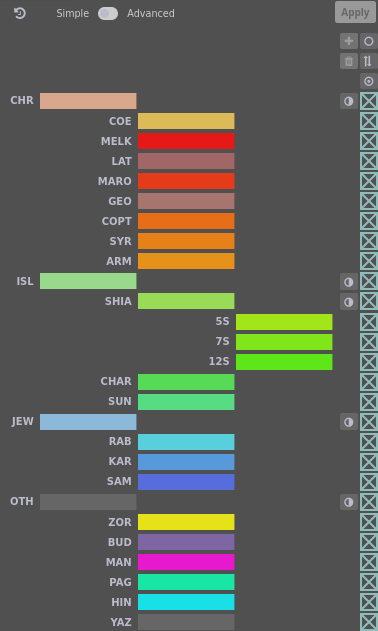
\includegraphics[height=9cm]{../src/assets/visualization-documentation/religion-hierarchy-1.png}%
  \hspace{1cm}
  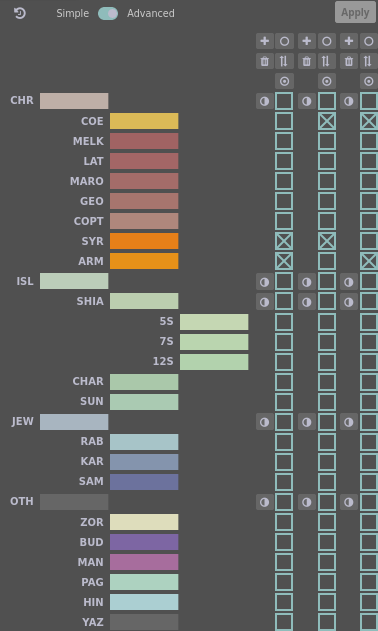
\includegraphics[height=9cm]{../src/assets/visualization-documentation/religion-hierarchy-2.png}
  \caption{\textbf{Left:}
    The religion hierarchy in its default state.
    At the top are the controls to revert the filter, the switch between simple and advanced filter mode, and the apply button.
    The religions are visualized as an indented tree, and are filtered by enabling the respective checkbox.
    \\
    \textbf{Right:}
    The religion hierarchy in advanced mode.
    The filter limits pieces of evidence to those from places where two or more of the Syriac Orthodox Church (SYR), the Armenian Church (ARM), and the Church of the East (COE) are present.
  }
  \customlabel{fig:religion-hierarchy-1}{ left}
  \customlabel{fig:religion-hierarchy-2}{ right}
\end{figure}

This view shows \textbf{all religious groups} contained in the database and allows for selecting and filtering the data according to religion.


\subsubsection{Content}
The list of religious groups is hierarchical and represented by a tree visualization:
each religious group occupies a line, which is indented according to its rank in the hierarchy.
In technical terms, the higher level is conceptualized as \emph{parent,} the respective lower levels as \emph{children.}

Each line consists of an \emph{abbreviation} for the religious group, a \emph{node,} displayed as a bar, with the color associated with the group, and a checkbox used for filtering.
Hovering with the mouse over the line displays a tooltip with the full name of the religious group and the number of pieces of evidence for the group based on the currently applied filters.

The general religious affiliation (e.g., Christianity) is on the first level of the hierarchy.
For other religions beside Christianity, Islam, and Judaism, we made the pragmatic choice to group them under the category \emph{Other.}

The religious groups each have a distinct color.
For Christianity (red), Islam (green), and Judaism (blue), religious groups belonging to these general religious affiliations have hues of the same color.
However, the difference between colors is limited because of the number of religious groups.
In \emph{confidence mode} (\cref{sec:settings-display-mode}), the bars of the groups are colored based on the average confidence of the represented data.

\paragraph{Details Regarding Coloring and Saturation.}
Depending on the options \emph{show filtered data} (\emph{all data} or \emph{only active}) as well as \emph{display mode} (\emph{religion} or \emph{confidence} mode) in the \emph{settings,} the coloring of the bars changes:

\begin{enumerate}
  \item \emph{Only active,} \emph{religion mode} \\
    A bar has only one color.
    If \emph{any} data related to a religious group is active, the bar has saturated colors;
    if all data related to a religious group is filtered out, the bar is shown in a less saturated color.

  \item \emph{All data,} \emph{religion mode} \\
    A bar can be divided into two parts, a saturated and a less saturated part.
    The less saturated part represents the relative amount of data currently filtered out.

  \item \emph{Only active,} \emph{confidence mode} \\
    A bar can be divided into several sections.
    Each section represents the relative amount of data with a certain level of confidence.

  \item \emph{All data,} \emph{confidence mode} \\
    A bar can be divided into two general parts:
    a saturated and a less saturated part, representing the data currently active or filtered out, respectively.
    Each part can have several sections, which each represent the relative amount of data with a certain level of confidence.
\end{enumerate}

The \emph{aspect of confidence} used for the visualization can be selected in the \emph{confidence view.}
There, the currently used aspect is indicated with an eye symbol below the column.


\subsubsection{Interaction}

\paragraph{Selection.}
Clicking on a line will \emph{select} the religious group.
This group will be highlighted, and other groups will be displayed in less saturated colors.
The data represented by the selection will be \emph{brushed,} and is \emph{linked} to related data in all views.
For instance, map glyphs in the \emph{map} representing pieces of evidence with the selected religion will be highlighted, other locations will be represented by less saturated colors.

\paragraph{Filtering.}
The checkbox of a religious group can be unchecked, which leads to filtering out this group throughout the entire visualization.
Depending on whether \emph{only active} or \emph{all data} mode is selected in the \emph{settings,} data that has been filtered out is either hidden or displayed in less saturated colors.

There are two basic modes for filtering by religion (more details further below):
In \emph{Simple} mode, pieces of evidence matching \emph{any} of the checked religions are shown.
In \emph{Advanced} mode, only pieces of evidence from places are shown, where checked \emph{combinations} of religions were present.
Note that, in both modes, the selection is not applied until the \emph{Apply} button is clicked, which is enabled once there are changes to the filter.

\subparagraph{Simple Mode.}
In \emph{simple} mode, data is filtered simply according to the checked or unchecked religions.
Initially, all religions are checked.
To filter out a religion, it can be unchecked in the checkbox column.

\subparagraph{Advanced Mode.}
\label{sec:religion-view-advanced-mode}
In \emph{advanced} mode, it is possible to filter not individual religions but different \emph{combinations} of religions.
For instance, analysis may require to show places where two or more of the following three religious groups exist together: the Syriac Orthodox Church (SYR), the Armenian Church (ARM), and the Church of the East (COE)---but not those places where only one of the three is present.
In this case, pieces of evidence are active if, for any combination, all religions of that combination are present at a place.

Different from \emph{simple} mode, there are multiple columns of checkboxes.
Each column represents a set of religious groups as described above.
To \emph{control} the filters in \emph{advanced} mode, columns can be added by using the plus button above each column.
Every column (except the last remaining one) can be deleted by pressing the delete button above the column.

The following procedure creates a filter corresponding to the analysis described above (\cref{fig:religion-hierarchy-2}):

\begin{itemize}
  \item Switch to \emph{advanced} mode.
  \item Create two additional columns by pressing the plus button.
  \item In the first column, check SYR and ARM.
  \item In the second column, check SYR and COE.
  \item In the third column, check ARM and COE.
  \item Click the \emph{Apply} button.
\end{itemize}

\emph{Note}: If only places should match the filter where \emph{all} of these three religious groups are present, only one column in \emph{advanced} mode is necessary with all three groups checked.
This must be understood as \enquote{pieces of evidence with COE \textbf{and} ARM \textbf{and} SYR.}
In turn, this differs from checking the three religious groups in \emph{simple} mode, which equals \enquote{pieces of evidence with COE \textbf{or} ARM \textbf{or} SYR.}

\paragraph{Filter Controls.}
A few additional utilities are available for managing the checkbox columns.
The controls for adding (plus button) and removing (trash can button) are already described in the \cref{sec:religion-view-advanced-mode}.
Importantly, columns can only be added in advanced mode, and the last remaining column cannot be removed.
The additional controls in the view are:

\begin{description}
  \item[Revert filters]
    This button is found in the top left corner of the view.
    Clicking it reverts the filters back to the state that is currently shown in the visualization;
    that is, all changes that are not \emph{applied} yet are discarded.
  \item[Uncheck all boxes in this column]
    This button is found at the top of each checkbox column.
    Clicking it will uncheck all boxes in the column.
  \item[Invert all boxes in this column]
    This button is found at the top of each checkbox column.
    Clicking it will invert all boxes in the column;
    that is, boxes that were checked are unchecked, and vice versa.
  \item[Check all boxes in this column]
    This button is found at the top of each checkbox column.
    Clicking it will check all boxes in the column.
  \item[Toggle subtree]
    This button is present to the \emph{left} of some of the checkboxes in each column;
    namely regarding religions that have \emph{children} in the hierarchy.
    Clicking the button will check or uncheck this religion and all its \emph{children} in the respective column.
    Whether clicking checks or unchecks depends on whether the majority of checkboxes in the subtree are checked.
\end{description}


\subsection{Timeline}
\label{sec:timeline}

\begin{figure}[tb]%
  \centering%
  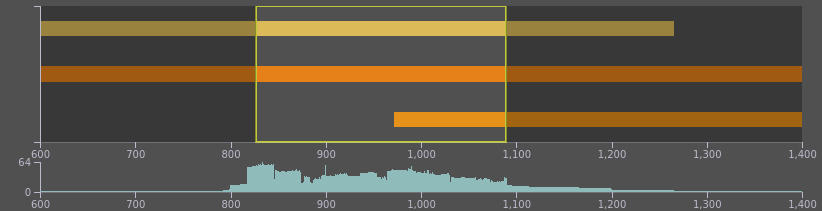
\includegraphics[width=0.8\textwidth]{../src/assets/visualization-documentation/timeline-1.png}\\\vspace{0.5cm}
  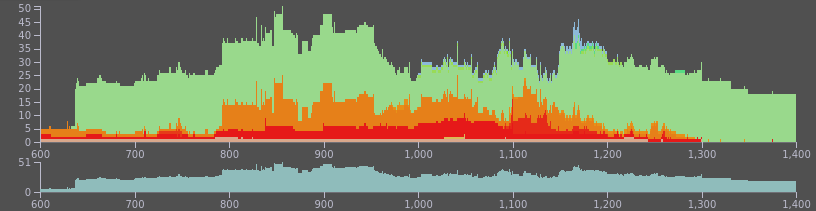
\includegraphics[width=0.8\textwidth]{../src/assets/visualization-documentation/timeline-2.png}%

  \caption{\textbf{Top:}
    The timeline in qualitative mode, showing three religious groups.
    A time range between 830 and 1090 is set as the filter.
    \\
    \textbf{Bottom:}
    The timeline in qualitative mode.
  }
  \customlabel{fig:timeline-1}{ top}
  \customlabel{fig:timeline-2}{ bottom}
\end{figure}

The \emph{Timeline} shows the distribution of the different religious groups \textbf{along the overall time period:} 600--1400 CE.
In \emph{confidence mode,} the level of confidence is shown instead of religious groups (\cref{sec:confidence,sec:settings-pane}).


\subsubsection{Content}

The \emph{timeline} consists of two graphs:
the \textbf{\emph{main timeline}} and a smaller \textbf{\emph{overview.}}
The graphs are described in the following.

Also, the view changes depending on the choice of \emph{show filtered data} in the \emph{settings} (\cref{sec:settings-pane}):
in \emph{all data} mode, data that has been filtered out is indicated by less saturated colors.
In \emph{only active} mode, data that has been filtered out is hidden from the visualization in all views, including the timeline.

\paragraph{Main Timeline.}
The \emph{main timeline} shows either a qualitative summary or quantitative information, depending on the \emph{timeline mode} selected in the \emph{settings pane.}
If \emph{quantitative} is selected, the number of pieces of evidence of that type in that year is encoded into the height of the area as a \emph{stacked area chart.}
If \emph{qualitative} is selected, the timeline only shows \emph{whether} there is evidence of that type each year.
The colors used in the graph match the ones used in the \emph{religion view} or \emph{confidence view,} depending on the \emph{display mode} selected in the \emph{settings pane.}
Importantly, the \emph{main timeline} can be used to filter the data according to time (\cref{sec:timeline-filtering}).


\paragraph{Overview.}
The smaller \textbf{overview} serves as a \emph{minimap} for the larger \emph{main timeline:}
it always shows the entire time range contained in the database.
By clicking and dragging in the \emph{overview,} a rectangle can be drawn which represents a time range.
The \emph{main timeline} \emph{zooms} to this time range and shows data in greater detail.
The overview represented by the lower graph does not change during this \emph{zooming} in the upper graph.
Vice versa, if the data is filtered by clicking and dragging in the \emph{main timeline} (see \enquote{Filtering} (\cref{sec:timeline-filtering}), the selected range is indicated as a thick bar below the \emph{overview.}

The rectangle representing the time range for zooming can be moved by clicking and dragging or altered by changing the width of the rectangle.
Note the mouse cursor in form of a grabbing hand (or a four-headed arrow) when hovering over the rectangle or the double-headed arrow when hovering the left and right borders of the rectangle, respectively.
Clicking anywhere in the \emph{overview} outside the rectangle will deactivate the zooming.

\paragraph{Tooltips.}

When \textbf{hovering} over any of the graphs, a tooltip with a summary of pieces of evidence for that year is displayed.
If the \emph{main timeline} shows a smaller time range than the \emph{overview,} the year in the tooltip depends on whether the mouse cursor is on the \emph{main timeline} or the \emph{overview.}

When \textbf{selecting} data in other views, through \emph{brushing and linking,} only the selected data shows in the timeline.
\emph{Note:} Selecting data in the timeline itself is not possible.

\subsubsection{Interaction}

\paragraph{Filtering.}
\label{sec:timeline-filtering}
By \emph{clicking and dragging} in the \emph{main timeline,} a rectangle can be drawn which represents a time range.
Data outside the time range is filtered out;
accordingly, the area outside the rectangle is displayed in less saturated colors.
The time range serves as a time filter for the data across all views.

The rectangle representing the time range for filtering can be moved by clicking and dragging or altered by changing the width of the rectangle.
Note the mouse cursor in form of a grabbing hand when hovering over the rectangle or the double-headed arrow when hovering the left and right borders of the rectangle, respectively.
Clicking anywhere in the \emph{main timeline} resets the filter.


\subsection{Untimed Data}
\label{sec:untimed-data}

Data with \textbf{missing temporal information} cannot be included in the timeline.
Accordingly, this data is visualized in the \emph{untimed data view} as a stacked bar chart.

\subsubsection{Content}

The chart is divided by the four general religious affiliations along the x-axis.
All pieces of evidence that have no temporal information and belong to one of these religious affiliations are stacked, with the number of pieces of evidence on the y-axis.
The pieces of evidence are grouped and colored according to the religious group or the level of confidence, depending on the \emph{display mode} selected in the \emph{settings pane} (\cref{sec:settings-pane}).

\emph{Note:} Missing data is normal during research and while entering data is still in progress.
However, missing data can severely affect confidence in the visualization if not properly communicated.
We have therefore chosen to make missing geographical locations and time information explicit in separate views of this interface (apart from \emph{untimed data,} see \emph{\enquote{unplaced data}} in the \emph{location list} (\cref{sec:location-list-unplaced})).
This also allows for searches directed at data in need of improvement.


\subsection{Confidence View}
\label{sec:confidence}

\begin{figure}[tb]
  \centering
  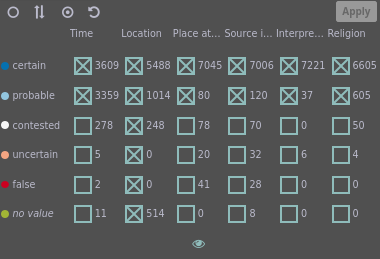
\includegraphics[width=0.35\textwidth]{../src/assets/visualization-documentation/confidence.png}
  \caption{
    The confidence view.
    Aspects of confidence are listed as columns, and confidence levels ordered into rows.
    Checkboxes control which confidence levels should be shown for each aspect, and the number of pieces of evidence for each confidence level and aspect are given.
  }
  \label{fig:confidence}
\end{figure}

This view shows the different \textbf{levels of confidence} attributed to the different elements of a piece of evidence (i.e., place, religious group, time span, etc.).

\subsubsection{Contents}

The view consists of a table, in which each row represents one \textbf{level of confidence} and each column an \textbf{aspect of confidence.}

For each cell in the table, a \textbf{checkbox} for filtering (\cref{sec:confidence-filtering}) is displayed as well as the \textbf{number of pieces of evidence} with the respective confidence and aspect.
The rows are sorted by descending level of confidence.

\paragraph{Levels of Confidence.}
Generally, the confidence of any given information was categorized according to these 5 degrees:

\begin{itemize}
  \item \emph{certain} (blue),
  \item \emph{probable,}
  \item \emph{contested,}
  \item \emph{uncertain,} and
  \item \emph{false} (red).
\end{itemize}

In addition, a confidence can have \emph{no value} at all (green).

\label{sec:confidence-note-no-place-confidence-value}
\emph{Note:} The attribution with \emph{no value} is used while data is still being collected and usually does not appear in a published instance of this visualization.
A notable exception are places, especially regions, with no geographical coordinates.
In that case, no attribution of confidence except \emph{no value} is suitable.

\paragraph{Aspects of Confidence.}
Confidence is attributed to different aspects of the data:

\begin{description}
  \item[Timespan confidence]
    signifies the confidence in the veracity of the timespan stored in a piece of evidence.
    Pieces of evidence without a time attribute are assigned the confidence \emph{no value.}
  \item[Confidence of location]
    signifies the confidence in the geographical location of a place.
    Some places, especially regions, have \emph{no value} (\cref{sec:confidence-note-no-place-confidence-value}).
  \item[Confidence of place attribution]
    signifies the confidence in assigning a location from the database to a toponym from a source.
  \item[Confidence regarding the source]
    signifies the confidence in the veracity and objectivity of the source itself regarding a piece of evidence.
  \item[Confidence of interpretation]
    signifies the confidence in the correct interpretation and recording of the source when entering a piece of evidence into the database.
  \item[Confidence regarding religion]
    signifies the confidence in the veracity of the presence of a particular religious group at a given time and place.
\end{description}


\subsubsection{Interaction}

\paragraph{Filtering.}
\label{sec:confidence-filtering}
For each aspect of confidence and each confidence level, a checkbox is shown in the respective cell.
Unchecking a checkbox will filter out pieces of evidence with this confidence level for that aspect of confidence.
This allows for a very fine-grained control over what data to visualize.

Note that the selection is not applied until the \emph{Apply} button is clicked.
This button is disabled if the selected filters are matching the data currently visualized.

The filters work in \emph{logical conjunction} across different aspects of confidence;
that is, having filters in place for multiple aspects of confidence will only show pieces of evidence that match \emph{all} filters.

Four additional buttons in the top left corner make filtering more convenient:

\begin{enumerate}
  \item Uncheck all checkboxes.
  \item
    Invert all checkboxes.
    Checked boxes are unchecked, unchecked boxes are checked.
  \item Check all checkboxes.
  \item
    Revert the selection of checkboxes to the default.
    By default, \emph{all} confidence levels are selected for confidence of location, and only \emph{certain} and \emph{probable} for the other confidence aspects.
\end{enumerate}

In addition, entire \emph{rows} or \emph{columns} of checkboxes can be set to either checked or unchecked by clicking the \emph{row header} (the confidence levels) or the \emph{column header} (the aspects of confidence).
Here, the new value for the new row (or column) is the inverse of what the majority of values (3 or more) was before;
for example, if 4 checkboxes were checked and 2 unchecked for the \emph{uncertain} row, clicking on the row header would \emph{uncheck} all checkboxes in the row.

\paragraph{Visualized Aspect of Confidence.}
By clicking on the eye in the bottom row of each column, the aspect of confidence that is visualized in \emph{Confidence} mode (\cref{sec:settings-display-mode}) can be selected.
The currently selected aspect is indicated by a colored eye.
By default, \emph{confidence regarding religion} is used.


\subsection{Source View}
\label{sec:source}

\begin{figure}[tb]
  \centering
  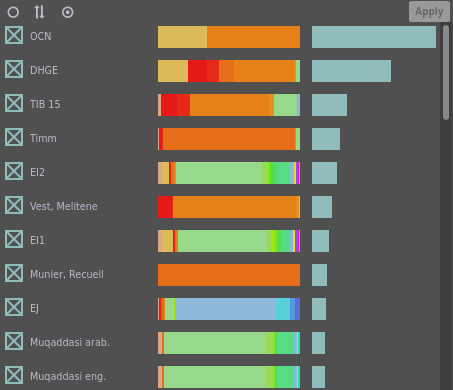
\includegraphics[width=0.4\textwidth]{../src/assets/visualization-documentation/source.png}
  \caption{
    The source view.
  }
  \label{fig:source}
\end{figure}

This view shows the \textbf{sources} from which the pieces of evidence (i.e., sets of data concerning a place, religious group, time span, and the respective confidences) were gathered.

\subsubsection{Contents}

The view consists of a table, in which each row represents one source.
The rows are sorted by descending number of pieces of evidence.
Note that a piece of evidence can stem from more than one source;
therefore, the sum total of all references to sources can be larger than the sum total of pieces of evidence.
In what follows, the respective columns of one given row are described.

\paragraph{Checkboxes.}
The first column contains a \emph{checkbox} that toggles the visibility of evidence from a source.
Keep in mind that a piece of evidence can stem from more than one source:
as long as \emph{any} source associated with a piece of evidence is checked in this view, the piece of evidence will be active.


\paragraph{Short Names.}
The second column shows the \textbf{short name} of the source, generally an abbreviation.
The full name of the source with bibliographical details is available via a tooltip;
that is, when hovering over the name with the mouse.


\paragraph{Religion/Confidence Segmentation Visualization.}
The third column visualizes the segmentation of the pieces of evidence on the religions or on the levels of confidence, depending on the chosen \emph{display mode} (\cref{sec:settings-display-mode});
in \emph{confidence mode,} instead of religion, the currently selected aspect of confidence is used).
The visualization used is a normalized stacked bar chart.
Because the total width of the bars is the same regardless of the amount of pieces of evidence, the width of each segment signifies the number of pieces of evidence with that religion or confidence level \emph{in relation to} the total evidence count for that source.


\paragraph{Evidence Count Visualization.}
The fourth column visualizes the count of pieces of evidence for each source.
This column uses the same scaling in all rows:
the longer the bar, the more pieces of evidence stem from the respective source.
This effectively creates a vertical histogram across the rows.

\subsubsection{Interaction}

\paragraph{Selection.}
Clicking on a row will \emph{select} the source, \emph{brush} the represented data, and \emph{link} related data in all views.
For instance, locations in the \emph{map} with pieces of evidence from the selected source will be highlighted, other locations will be represented by less saturated colors.
Clicking on the same row again will reset the selection.
Selecting a different row, or an element in a different view, will replace the selection;
that is, only one source can be selected at a time.

\paragraph{Filtering.}
A source can be filtered out from the visualized data in all views by (un-)checking the respective checkbox.
Note that the new filter is not applied until the \emph{Apply} button is clicked.
This button is disabled if the selected filters are matching the data currently visualized.

Checking multiple (or all) sources works as a \emph{logical disjunction:}
a piece of evidence is matched if it stems from \emph{any} of the checked sources.

The source filter works together with filters from other views in \emph{logical conjunction;}
for instance, if only source X and religion Y are set active in the respective views, only pieces of evidence with source X \emph{and} religion Y are matched.

Three additional buttons in the top left corner make filtering more convenient:

\begin{enumerate}
  \item Uncheck all checkboxes.
  \item
    Invert all checkboxes.
    Checked boxes are unchecked, unchecked boxes are checked.
  \item Check all checkboxes.
\end{enumerate}

\paragraph{Sorting.}
The order of the shown sources can be changed using the sorting options switch in the center of the header of the view.
The two options are:

\begin{enumerate}
  \item Sort the sources first alphabetically, in ascending order, by their short name, which is shown in the second column of the list.
  \item Sort the sources first in descending order by the number of visible pieces of evidence derived from them.
\end{enumerate}

For both sorting modes, the other sorting criterion is considered as secondary criterion.
More specifically, if the sources are ordered by count, and two sources have the same count, the source that would come first alphabetically is listed first of the two.


\subsection{Tag View}
\label{sec:tags}

\begin{figure}[tb]
  \centering
  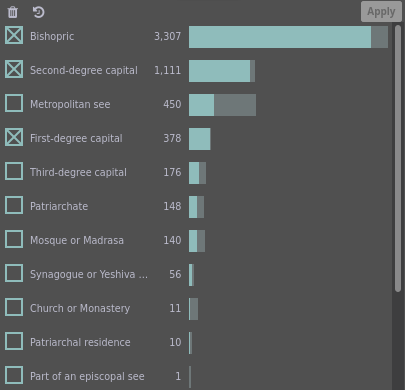
\includegraphics[width=0.4\textwidth]{../src/assets/visualization-documentation/tags.png}
  \caption{
    The tags view.
    Three tags were selected.
  }
  \label{fig:tags}
\end{figure}

This view shows \textbf{tags} which are associated with pieces of evidence (i.e., sets of data concerning a place, religious group, time span, and the respective confidences).
Tags were implemented to include additional information and to make further distinctions possible.
For instance, the tag \emph{Bishopric} is attributed to pieces of evidence referring to bishoprics as distinguished from \emph{metropolitan sees.}
This way, the visualized data can be filtered according to additional criteria.
Note that, by default, all tags are \emph{deselected.}
This means that no filters based on tags are active ((\cref{sec:tags-interaction}).


\subsubsection{Contents}

The view consists of a table, in which each row represents one tag.
The rows are sorted by descending number of pieces of evidence.
In what follows, the respective columns of one given row are described.

\begin{description}
  \item[Checkboxes]
    The first column contains a \emph{checkbox} used for filtering.

  \item[Tag Names]
    The second column shows the name of the tag.
    Generally, the name should be self-explanatory.
    Further information is displayed when hovering with the mouse.

  \item[Evidence Count Visualization]
    The third column visualizes the count of pieces of evidence for each source.
    The less saturated part of the bar represents pieces of evidence that are not active (i.e., do not match the current filters).
\end{description}

\subsubsection{Interaction}
\label{sec:tags-interaction}

\paragraph{Selection.}
Clicking on a row will \emph{select} the tag, \emph{brush} the represented data, and \emph{link} related data in all views.
For instance, locations in the \emph{map} with pieces of evidence with the selected tag will be highlighted, other locations will be represented by less saturated colors.
Clicking on the same row again will reset the selection.
Selecting a different row, or an element in a different view, will replace the selection.
Only one tag at a time can be selected.

\paragraph{Filtering.}
The visualized data can be filtered according to one tag or multiple tags in all views by (un-)checking the appropriate checkbox or checkboxes.
Keep in mind that a piece of evidence can have no tag, one tag, or multiple tags.
If, for instance, it has no tag, its visibility is not affected by the checkboxes.
If, on the other hand, it has multiple tags, its visibility is only affected by (un-)checking all respective checkboxes.
Note that the selection is not applied until the \emph{Apply} button is clicked.

Checking multiple (or all) tags works as a \emph{logical disjunction:}
a piece of evidence is matched if it is assigned \emph{any} of the checked tags.
The tag filter works together with filters from other views in \emph{logical conjunction:}
for instance, if only tag X and religion Y are selected in the respective views, only pieces of evidence with tag X \emph{and} religion Y are matched.

Two additional buttons in the top left corner make filtering more convenient:

\begin{enumerate}
  \item
    Uncheck all checkboxes;
    that is, remove all filters based on tags.
    Note that this is not applied until the \emph{Apply} button is clicked.

  \item Revert all checkboxes to represent the state of filters applied last.
\end{enumerate}


\section{GeoDB-Editor}

\todo[inline]{todo}

\section{Annotator}
\label{sec:annotator}

\todo[inline]{intro?}

\subsection{Database Schema}
\label{sec:database-schema}

\begin{figure}[htb]
  \centering
  \tikzset{
    table/.style = {
      minimum width=3.8cm,
      minimum height=1cm,
      rectangle,
      draw=black,
      node distance=0.2cm and 1.8cm
    },
    label/.style = {
      inner sep=1mm,
      pos=1,
      font=\ttfamily\footnotesize
    },
  }
  \begin{tikzpicture}
    [font=\ttfamily,-{Triangle[length=2mm,width=1.5mm]}]

    \node [table] (source) {source};
    \node [table,right=of source] (document) {document};
    \node [table,right=of document] (annotation) {annotation};
    \node [table,node distance=1.5cm and 1.8cm,below=of source] (sourcei) {source\_instance};
    \node [table,right=of sourcei] (reli) {religion\_instance};
    \node [table,below=of reli] (plai) {place\_instance};
    \node [table,below=of plai] (peri) {person\_instance};
    \node [table,below=of peri] (tg) {time\_group};
    \node [table,right=of reli] (rel) {religion};
    \node [table,right=of plai] (pla) {place};
    \node [table,right=of peri] (per) {person};
    \node [table,right=of tg] (ti) {time\_instance};
    \node [table,left=of peri] (ev) {evidence};

    \draw (document.west) to node[label,anchor=north west]{1} (source.east);
    \draw (annotation.west) to node[label,anchor=north west]{1} (document.east);
    \draw (sourcei) to node[label,anchor=north west]{1} (source);
    \draw (ev) to node[label,anchor=north west]{0..*} (sourcei);
    \draw (ev.east) to node[anchor=south east,label]{1} (reli.west);
    \draw (ev.east) to node[anchor=south east,label]{1} (plai.west);
    \draw (ev.east) to node[anchor=north east,label]{0..1} (peri.west);
    \draw (ev.east) to node[anchor=north east,label]{0..1} (tg.west);
    \draw (reli.east) to node[anchor=north east,label]{1} (rel.west);
    \draw (plai.east) to node[anchor=north east,label]{1} (pla.west);
    \draw (peri.east) to node[anchor=north east,label]{1} (per.west);
    \draw (tg.east) to node[anchor=north east,label]{0..*} (ti.west);

    \coordinate (as) at ($ (annotation.south) + (-90:0.7cm) $);
    \draw [rounded corners=3mm] (reli.east) -- ++(5mm,0) |- (as) -- (annotation.south);
    \draw [rounded corners=3mm] (plai.east) -- ++(6mm,0) |- (as) -- (annotation.south);
    \draw [rounded corners=3mm] (peri.east) -- ++(7mm,0) |- (as) -- (annotation.south);
    \draw [rounded corners=3mm] (tg.east) -- ++(8mm,0) |- (as) -- (annotation.south) node [label,anchor=north west] {4 $\times$ (0..1)};
  \end{tikzpicture}
  \caption{Database structure of tables directly involved in storing historical evidence and annotations.}
  \label{fig:annotator-schema}
\end{figure}

The data is stored in a relational database.
These are exceptionally efficient in the lookup and querying of specific attributes and subsets of data, as well as complex joins across attributes and tables, at the cost of the readability and intuitivity of the storage format.
In particular, storing relationships such as an \emph{optional} relationship, or a \emph{one-to-many} relationship, cannot be modeled in a straightforward way, but require intermediate tables.
The database structure is, therefore, a bit more complex and fragmented than the mental data model it represents.
Still, it is valuable to understand the data model, because the way evidence is generated from annotations and groups of annotations is based very closely on that model.

\Cref{fig:annotator-schema} shows a simplified \emph{entity-relationship diagram} of the tables in the database involved in evidence creation and annotations.
One piece of evidence \emph{must} contain a place and religion, and \emph{may} contain one person and one or more time spans.
In the database, this is represented by instance tuples, where each instance also stores meta-information specific to that tuple, such as a comment and confidence.
The instance tuples then point to the base entities (places, religions, persons), which only exist once.
The one or more time spans (time instances) are grouped by a singular time group.
The instances \emph{may} be linked to one annotation, such that an annotation can \emph{either} be for a place, religion, person, or set of time spans.
Each annotation is attributed clearly to one document, and each document to one source.
An evidence tuple can be derived from zero or more sources, which is coded via the source instance table.
In cases where an evidence was created using the annotator, there is only one source instance, whose source is the same as that of the document the annotations belong to.

An evidence created from the annotator, therefore, is a \emph{group} of two to four annotations, where one belongs to a place instance, one to a religion instance, zero or one to a person instance, and zero or one to a time group.
Evidences created, for example, using the GeoDB-Editor look exactly the same, except that their instances do not have a connected annotation.
For more information on the database structure, please reference \cref{fig:db-structure}.


\subsection{Document Selection}
\label{sec:document-selection}

\begin{figure}[htb]
  \centering
  \begin{tikzpicture}
    \node [inner sep=0.0pt,anchor=north west] at (0,0) {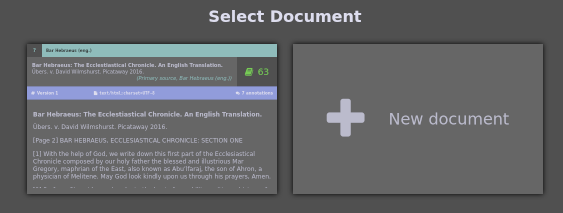
\includegraphics[width=281.5pt,height=106.5pt]{../src/assets/annotator-documentation/select-document.png}};
    \draw (-9.0pt,-15.5pt)
      node [anchor=east] {\footnotesize Document comment}
      [red!60!white]
      -- (13.5pt,-15.5pt)
      -- (22.5pt,-23.0pt);
    \draw (-9.0pt,-23.0pt)
      node [anchor=east] {\footnotesize Document ID}
      [red!60!white]
      -- (-9.0pt,-23.0pt)
      -- (13.5pt,-23.0pt);
    \draw (-9.0pt,-8.0pt)
      node [anchor=east] {\footnotesize Source ID}
      [red!60!white]
      -- (100.0pt,-8.0pt)
      -- (121.0pt,-31.5pt);
    \draw (-9.0pt,-30.5pt)
      node [anchor=east] {\footnotesize Source long name}
      [red!60!white]
      -- (13.5pt,-30.5pt);
    \draw (-9.0pt,-39.0pt)
      node [anchor=east] {\footnotesize Source type and short name}
      [red!60!white]
      -- (67.0pt,-39.0pt);
    \draw (-9.0pt,-45.5pt)
      node [anchor=east] {\footnotesize Document version}
      [red!60!white]
      -- (13.5pt,-45.5pt);
    \draw (-9.0pt,-53.0pt)
      node [anchor=east] {\footnotesize Document content type}
      [red!60!white]
      -- (41.0pt,-53.0pt)
      -- (46.0pt,-48.0pt);
    \draw (-9.0pt,-60.5pt)
      node [anchor=east] {\footnotesize Number of annotations}
      [red!60!white]
      -- (112.5pt,-60.5pt)
      -- (116.5pt,-48.5pt);
    \draw (-9.0pt,-78.0pt)
      node [anchor=east] {\footnotesize Document preview}
      [red!60!white]
      -- (13.5pt,-78.0pt);
    \draw (75.0pt,-109.0pt)
      node [anchor=north] {\footnotesize Click to open document}
      [red!60!white]
      -- (75.0pt,-90.0pt);
    \draw (212.0pt,-109.0pt)
      node [anchor=north] {\footnotesize Click to create new document}
      [red!60!white]
      -- (212.0pt,-90.0pt);
  \end{tikzpicture}

  \caption{
    The initial screen of the annotator shows a \emph{document selection,} where the document to be annotated can be selected.
    The documents are shown as cards, displaying additional metadata about the document and its underlying source.
    A separate link leads to a form for creating new documents.
  }
  \label{fig:document-selection}
\end{figure}

When opening the annotator, the first screen shows a list of all available documents, shown in \cref{fig:document-selection}.
Each document is represented by a card, which lists some metadata about the document and its source:

\begin{itemize}
  \item the ID of the source,
  \item the ID of the document,
  \item the name of the document (its comment field),
  \item the full name of the source,
  \item the type of the source (primary source, literature, ...),
  \item the short name of the source (e.g., \enquote{OCN}),
  \item the document version,
  \item the document content type,
  \item the number of annotations in that document,
  \item and a short preview of the document.
\end{itemize}

The goal of all that metadata is to make perfectly clear which document this is;
for example, there could be multiple \emph{versions} of one source, each being its own \emph{document.}
This could contain differences in spelling, whitespace, and other aspects, which in turn affect the positioning of existing annotations.
Therefore, creating new versions of existing documents when the textual content changes is favorable to updating the existing document, as that might create issues with those existing annotations.

To open a document in the annotator, simply \emph{click} on the card in question.
Besides one card for each existing document, there is also one card at the very end of the list to create a new document.
This will link to the document creation form, described in \cref{sec:document-creation}.


\subsection{Creating a new Document}
\label{sec:document-creation}

Creating a new document is fairly simple:
This will show a page with a form, the contents of which will then populate a new record in the \verb!document! table.
The form has five fields, all of them mandatory, described below:

\begin{description}
  \item[Source:]
    Each document is attributed to a source, which can be selected here using a drop-down menu.
    The source entry must already exist when creating a new document.

  \item[Version:]
    A source can have multiple versions of itself as documents, and so each document must have a version number.
    This number \textbf{must be} unique for each source (i.e., no two documents of the same source may have the same version), and only numerical values are allowed.

  \item[Comment:]
    This field is the title of the document.
    Currently, this is a bit badly named and configured on my part, as \emph{\enquote{comment}} does not really fit the purpose of the field: providing a short and ideally unique and recognizable label for a document.
    On that note, the comment field is currently not enforced to be unique, but it might be favorable to give each document a unique comment in any case.
    I will at some point clean this up.

  \item[Content type:]
    For the moment, annotatable documents can only have two \emph{content types:}
    either, they are just plain text, or they are marked-up hypertext (HTML).
    There are subtle differences in how to calculate text positions between plain text (where each character in the file is visible) and HTML.
    In HTML, a character in the file might have a special meaning, such as making the following text bold, or forcing a line break.
    This field is a drop-down menu with those two options.
    It is important to select the correct one here to avoid strange effects during annotation.

  \item[Content:]
    This is a file selection form field.
    Select the file containing the document text from your hard drive, and its contents will be uploaded and put in the database when submitting the form.
    By default, the file selection dialog should only show text and HTML files.\\
    \textbf{Note:} The file you select here will be read by the browser and sent to the server.
    This is one of the few occasions where the browser is allowed to read your files, or at least one of them.
    Be careful not to select any confidential or private file by accident, as its contents will be visible to other users of the annotator as well.
\end{description}

After filling out all fields properly, a new document is created by clicking on the green \emph{Submit} button.
This will put the document in the database and navigate back to the document selection page (see \cref{sec:document-selection}).
Before clicking the button, no data will be sent to the server, and you can clear all form fields by clicking on the gray \emph{Reset form} button.


\begin{figure}[htb]
  \centering
  \begin{minipage}{6cm}
    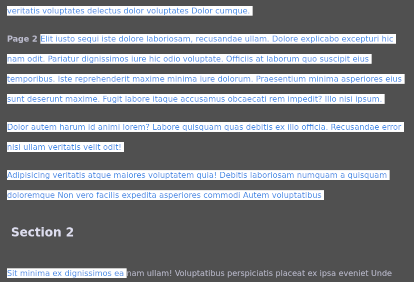
\includegraphics[width=\textwidth]{../src/assets/annotator-documentation/virtual-text.png}
  \end{minipage}%
  \quad%
  \begin{minipage}{9cm}
    \lstset{%
      basicstyle={\scriptsize\ttfamily},
      language=html5,
      showspaces=false,
      showstringspaces=false,
      keywordstyle=\color{blue}\bfseries,
      ndkeywordstyle=\color{green!40!black}\bfseries,
      stringstyle=\color{brown!80!black},
    }
    \begin{lstlisting}
...
<p>
  <strong data-virtual-text="Page 2 "></strong>Elit...
  Dolore explicabo excepturi hic nam odit.
  ...
</p>
...
<h2 data-virtual-text="Section 2"></h2>
<p>
  Sit minima ex dignissimos ea nam ullam!
  ...
</p>
...
    \end{lstlisting}
  \end{minipage}

  \caption{
    (l) Virtual text in a document cannot be selected, and is not part of annotations.
    Virtual text can be placed inline, or as a block element.
    (r) The HTML source code to produce the virtual text on the left.
  }
  \label{fig:virtual-text}
\end{figure}


In theory, all HTML files should be fine to use for annotation purposes.
For security purposes, many tag types and tag attributes are stripped from the document before upload\footnote{%
  The entirety of \texttt{<script>}, \texttt{<style>}, and \texttt{<head>} tags are discarded, both their content and the DOM nodes themselves.
  Disallowed tags are removed, but their contents are kept as plain text and child nodes.
  Allowed tags are:
  \texttt{<a>}, \texttt{<abbr>}, \texttt{<address>}, \texttt{<article>},
  \texttt{<aside>}, \texttt{<b>}, \texttt{<bdi>}, \texttt{<bdo>}, \texttt{<blockquote>},
  \texttt{<br>}, \texttt{<caption>}, \texttt{<cite>}, \texttt{<code>}, \texttt{<col>},
  \texttt{<colgroup>}, \texttt{<dd>}, \texttt{<del>}, \texttt{<details>}, \texttt{<dfn>},
  \texttt{<div>}, \texttt{<dl>}, \texttt{<dt>}, \texttt{<em>}, \texttt{<figcaption>},
  \texttt{<figure>}, \texttt{<footer>}, \texttt{<h1>}, \texttt{<h2>}, \texttt{<h3>},
  \texttt{<h4>}, \texttt{<h5>}, \texttt{<h6>}, \texttt{<header>}, \texttt{<hr>},
  \texttt{<i>}, \texttt{<img>}, \texttt{<ins>}, \texttt{<kbd>}, \texttt{<li>},
  \texttt{<main>}, \texttt{<mark>}, \texttt{<nav>}, \texttt{<ol>}, \texttt{<p>},
  \texttt{<picture>}, \texttt{<pre>}, \texttt{<q>}, \texttt{<rp>}, \texttt{<rt>},
  \texttt{<ruby>}, \texttt{<s>}, \texttt{<samp>}, \texttt{<section>}, \texttt{<small>},
  \texttt{<span>}, \texttt{<strong>}, \texttt{<sub>}, \texttt{<summary>}, \texttt{<sup>},
  \texttt{<table>}, \texttt{<tbody>}, \texttt{<td>}, \texttt{<tfoot>}, \texttt{<th>},
  \texttt{<thead>}, \texttt{<time>}, \texttt{<title>}, \texttt{<tr>}, \texttt{<u>},
  \texttt{<ul>}, and \texttt{<wbr>}.
  All attributes are removed from tags, except for
  \texttt{href}, \texttt{title} and \texttt{hreflang} for \texttt{<a>} tags;
  and \texttt{src}, \texttt{width}, \texttt{height}, \texttt{alt}, and \texttt{title} for \texttt{<img>} tags.
  In addition, the \texttt{data-virtual-text} attribute can be placed on every tag.
}.
The resulting document in the database will consist of semantically relevant, but unstyled, HTML tags, and text.
However, there might be special considerations to be made about how you want the text to be represented.
Some questions to think about before creating a HTML document for annotation are:

\begin{itemize}
  \item
    Are there sections of the text (e.g., page numbers) that are \emph{\enquote{not really}} part of the text?
    That means: those sections should not be selectable or annotatable.
    Some information on how to incorporate virtual text is given in the paragraph below.
  \item
    Is there text that requires special highlighting or styling?
    Would such styling interfere with the styling of annotated text or the evidence links?
  \item
    Is the text left-to-right (e.g., latin scripts), right-to-left (e.g., Arabic), or even top-to-bottom, right-to-left (e.g., Chinese)?
    Is the writing direction mixed (e.g., English headings in Arabic text)?
\end{itemize}

To add \emph{virtual} text to a document, we use HTML \emph{pseudo-elements,} which are generated by the browser and are not part of the textual content of the document.
Take note that virtual text, therefore, is only possible to add when using HTML, not plain text.
Virtual text has the advantage of being skipped by the offset calculations and not being selected, therefore also not being part of the text selection and the annotation content.
For adding virtual text, add the respective HTML element (e.g., \verb!<h2>! or \verb!<span>!) \emph{without} any text between the tags.
The virtual text itself needs to be passed as an \emph{element attribute} to the text.
The attribute name used is \verb!data-virtual-text!.
The appearance of the virtual text depends on which type of HTML element you use to represent it.
Block-level elements, like headings (\verb!<h1>!, \verb!<h2>!, etc.), will be represented thus, and inline elements, like \verb!<span>!, \verb!<strong>!, or \verb!<em>!, will be placed inline, which might be useful if the virtual text should be within a paragraph (e.g., for sentence numbering).
\Cref{fig:virtual-text} shows an example document with two instances of virtual text:
One inline \verb!<strong>! element, and one block-level \verb!<h2>! element.
The HTML content of the document to produce this effect looks as listed in \cref{fig:virtual-text}.


\subsection{Annotations}
\label{sec:annotations}

An \emph{annotation,} in general, consists of a \emph{start} and \emph{end} position within a \emph{document,} as well as an \emph{instance} (see \cref{sec:database-schema} for more details).
Annotations are represented in the text by colored background behind the annotated text passage.
In the following, the user controls of the annotator are described, as well as how to create, edit, and delete annotations.


\subsubsection{The Annotator Interface}
\label{sec:annotation-annotator}

\begin{figure}[htb]
  \centering
  \begin{tikzpicture}
    \node [inner sep=0.0pt,anchor=north west] at (0,0) {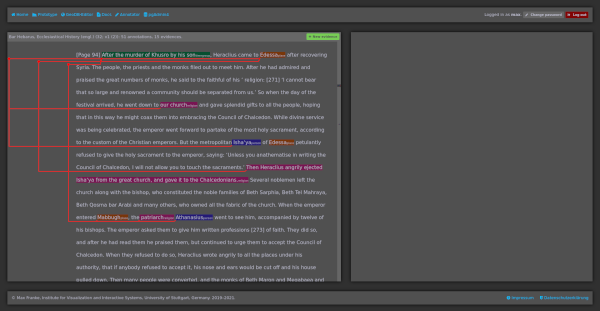
\includegraphics[width=300.0pt,height=155.5pt]{../src/assets/annotator-documentation/annotator-interface.png}};
    \draw (-9.0pt,-8.0pt)
      node [anchor=east] {\footnotesize New evidence button}
      [blue!40!white]
      -- (144.5pt,-8.0pt)
      -- (153.0pt,-16.5pt);
    \draw (-9.0pt,-18.5pt)
      node [anchor=east] {\footnotesize Document information}
      [blue!40!white]
      -- (6.5pt,-18.5pt);
    \draw (-9.0pt,-30.5pt)
      node [anchor=east] {\footnotesize Document area}
      [blue!40!white]
      -- (2.5pt,-30.5pt);
    \draw (-9.0pt,-62.5pt)
      node [anchor=east] {\footnotesize Annotation}
      [blue!40!white]
      -- (89.0pt,-62.5pt)
      -- (89.0pt,-53.5pt);
    \draw (-9.0pt,-83.5pt)
      node [anchor=east] {\footnotesize Evidence link}
      [blue!40!white]
      -- (19.0pt,-83.5pt);
    \draw (-9.0pt,-119.5pt)
      node [anchor=east] {\footnotesize Swimlanes}
      [blue!40!white,-Circle]
      -- (13.5pt,-119.5pt)
      -- ++(5.0pt,5.0pt);
    \draw (-9.0pt,-127.0pt)
      node [anchor=east] {\footnotesize Text area}
      [blue!40!white,-Circle]
      -- (63.5pt,-127.0pt)
      -- ++(7.5pt,7.5pt);
    \draw (-9.0pt,-134.5pt)
      node [anchor=east] {\footnotesize Scrollbar}
      [blue!40!white]
      -- (169.5pt,-134.5pt);
    \draw (225.0pt,-160.0pt)
      node [anchor=north] {\footnotesize Editor pane}
      [blue!40!white,circle]
      -- (225.0pt,-80.0pt);
  \end{tikzpicture}

  \caption{
    The annotator consists of of two main components:
    the \emph{document area} on the left, and the \emph{editor pane} on the right.
    A section on the top displays information about the current document.
    Annotations are displayed by colored background behind the annotated text.
    Evidence is represented by links connecting multiple annotations.
    The evidence is ordered into vertical pathways on the left of the document area, so-called \emph{swimlanes.}
  }
  \label{fig:annotator-interface}
\end{figure}

After having selected a document in the document selection screen (\cref{sec:document-selection}), it and its annotations and evidences are displayed in the annotator.
The annotator interface, shown also in \cref{fig:annotator-interface}, consists of two main views.
The \emph{document area} on the left shows the document, annotations, and evidences;
and the \emph{editor pane} on the right shows annotation and evidence editors, when open.

The document area is scrollable, and the document text is displayed here with a large line height to accomodate links between the rows.
A scrollbar on the left of the document area shows the current position in the document, and the positions of annotations are also indicated here.
Annotations within the text are indicated by a colored background, where different colors signify different types of annotations (place, person, religion, time group).

Evidences are groups of one place annotation, one religion annotation, zero or one person annotations, and zero or one time group annotations (see \cref{sec:database-schema}).
In the annotator, they are represented by a line connecting all annotations that are part of the evidence.
If the annotations are in different lines of the text, the line takes a detour via the left margin of the document to avoid crossing text.
In the margin, the evidence links are horizonally distributed into \emph{swimlanes} to avoid overdrawing.
For multiple evidence links going into the same line of text, they are also vertically distributed in the same fashion.

The editor pane is where the annotation or evidence editor is displayed when creating or editing an annotation.
This is described in more detail below.
Initially, the editor pane is empty, as no annotation or evidence is being edited.


\subsubsection{Creating an Annotation}
\label{sec:annotation-creation}

\begin{figure}[htb]
  \centering
  \begin{tikzpicture}
    \node [inner sep=0.0pt,anchor=north west] at (1.0pt,-1.0pt) {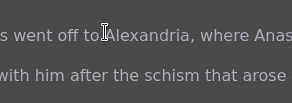
\includegraphics[width=146.0pt,height=51.5pt]{../src/assets/annotator-documentation/create-annotation-1.png}};
    \node [inner sep=0.0pt,anchor=north west] at (151.0pt,-1.0pt) {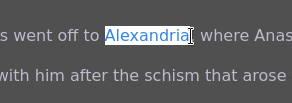
\includegraphics[width=146.0pt,height=51.5pt]{../src/assets/annotator-documentation/create-annotation-2.png}};
    \node [inner sep=0.0pt,anchor=north west] at (75.0pt,-255.0pt) {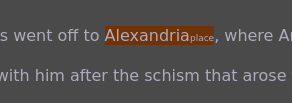
\includegraphics[width=146.0pt,height=51.5pt]{../src/assets/annotator-documentation/create-annotation-4.png}};

    \begin{scope}
      \clip (0.0pt,-75.0pt) --
        (175.0pt,-75.0pt) -- ++(-30.0pt,-70.0pt) -- ++(10.0pt,-20.0pt) -- ++(-30.0pt,-70.0pt)
        -- (0.0pt,-235.0pt) -- (0.0pt,-75.0pt);
      \node [inner sep=0.0pt,anchor=north west] at (0.0pt,-75.0pt) {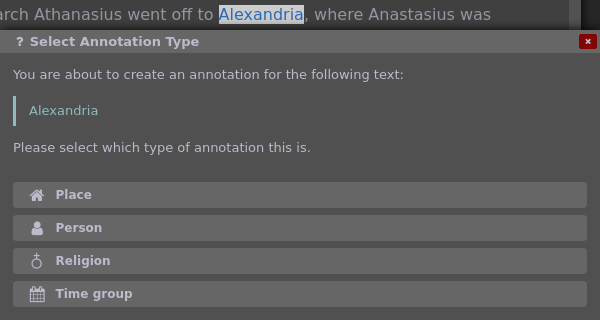
\includegraphics[width=300.0pt,height=160.0pt]{../src/assets/annotator-documentation/create-annotation-3a.png}};
    \end{scope}

    \begin{scope}
      \clip (300.0pt,-75.0pt) --
        (175.0pt,-75.0pt) -- ++(-30.0pt,-70.0pt) -- ++(10.0pt,-20.0pt) -- ++(-30.0pt,-70.0pt)
        -- (300.0pt,-235.0pt) -- (300.0pt,-75.0pt);
      \node [inner sep=0.0pt,anchor=north west] at (0.0pt,-75.0pt) {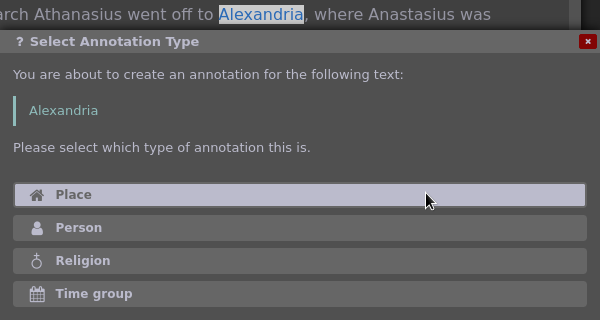
\includegraphics[width=300.0pt,height=160.0pt]{../src/assets/annotator-documentation/create-annotation-3b.png}};
    \end{scope}

    \draw [very thick,cyan!80!white!60!black] (175.0pt,-75.0pt) -- ++(-30.0pt,-70.0pt) -- ++(10.0pt,-20.0pt) -- ++(-30.0pt,-70.0pt);
    \foreach \x/\y/\r in {
      150.0pt/-25.5pt/0,
      150.0pt/-62.5pt/-90,
      150.0pt/-155.0pt/0,
      150.0pt/-245.0pt/-90%
    } {
      \begin{scope}[xshift=\x,yshift=\y,rotate=\r]
        \draw [fill=cyan!80!white!60!black,draw=none] (6.25pt,0.0pt) -- ++(-7.5pt,7.5pt) -- ++(0.0pt,-3.75pt) -- ++(-5.0pt,0.0pt) -- ++(0.0pt,-7.5pt) -- ++(5.0pt,0.0pt) -- ++(0.0pt,-3.75pt) -- cycle;
      \end{scope}
    }

    \draw [white,Bar->] (53.0pt,-11.0pt)
      node [anchor=south west,font=\sffamily\tiny] {Click \& drag}
      -- (74.0pt,-11.0pt);
    \draw [white,Bar-{>}.{Bar}] (203.0pt,-11.0pt)
      -- (247.0pt,-11.0pt)
      node [anchor=south east,font=\sffamily\tiny] {Release};
  \end{tikzpicture}

  \caption{
    Annotation creation starts by selecting a text passage using the mouse.
    Then, a dialog window pops up, where the type of annotation is selected.
    After editing and saving the new annotation, it appears in the text.
  }
  \label{fig:create-annotation}
\end{figure}

The process for creating a new annotation is shown in detail in \cref{fig:create-annotation}.
Initially, the text passage that is to be annotated needs to be selected using \emph{regular text selection;}
that is, going over the start of the text passage with the mouse, push and hold down the left mouse button, drag the mouse until the end of the text passage, and release the left mouse button.
The selection should become highlighted while doing this.

As soon as you release the left mouse button, the selection of the text passage is finished.
The selected text is what will become the annotation.
Because there are four types of annotations, depending on which type of instance is represented (see \cref{sec:database-schema}), next a pop-up window appears, where the type of annotation needs to be selected.
The window also shows the content of the annotation again, and there are four buttons, one for each type of annotation.
By clicking one of the buttons, that type is selected, the pop-up window is closed, and the \emph{annotation editor} is opened.
If you want to re-select the text passage or abort the creation of the annotation for any other reason, you can either click on the red cross in the top right, or anywhere outside of the pop-up window.

Next, in the \emph{editor pane,} an annotation editor appears, where you can fill out the data for that annotation and the connected instance.
This editor window is described in more detail in \cref{sec:annotation-editing}, as the process for creating and editing existing annotations is quite similar.
The only difference is that:

\begin{enumerate}
  \item the button for closing the editor will cancel creation without a prompt,
  \item the delete button at the bottom is instead labeled \emph{\enquote{Cancel creation}} and serves the same function,
  \item the save button at the bottom is instead labeled \emph{\enquote{Create}} and clicking it will persist the new annotation and instance to the database, and
  \item the editor row for changing the text extent of the annotation is missing.
\end{enumerate}

Finally, after clicking \emph{\enquote{Create}} in the editor, the editor will close, and the new annotation will appear in the document.
Annotations \emph{may} overlap, and may even cover exactly the same text passage.
It is completely fine to do a text selection over an existing annotation in the text.
When annotations overlap, the parts where they do are highlighted in gray instead of the normal annotation colors.

\begin{figure}[htb]
  \centering
  \begin{tikzpicture}
    \node [inner sep=0.0pt,anchor=north west] at (0,0) {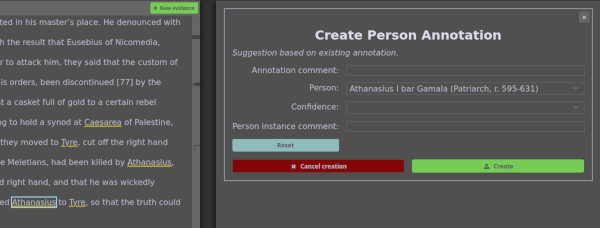
\includegraphics[width=300.0pt,height=114.0pt]{../src/assets/annotator-documentation/annotation-suggestion.png}};
    \draw (25.0pt,-123.0pt)
      node [anchor=west] {\footnotesize Annotation suggestion}
      [red!60!white]
      -- (20.0pt,-123.0pt)
      -- (15.0pt,-105.0pt);
    \draw (310.0pt,-27.0pt)
      node [anchor=west] {\footnotesize Suggestion source}
      [red!60!white]
      -- (205.0pt,-27.0pt);
    \draw (310.0pt,-45.5pt)
      node [anchor=west] {\footnotesize Pre-selected entity}
      [red!60!white]
      -- (280.0pt,-45.5pt);
  \end{tikzpicture}
  \caption{
    Suggestions for new annotations are indicated by yellow curly underlining.
    These suggestions are based on known names for entities from the database, as well as existing annotation content.
  }
  \label{fig:annotation-suggestion}
\end{figure}

The server will also generate suggestions for annotations.
These are based on known names (place names, alternative names from other languages, religion and person names) from the database, as well as on existing annotations in the current document.
\Cref{fig:annotation-suggestion} shows an example:
The person \emph{Athanasius I bar Gamala} has been annotated in the text previously (under the name \emph{\enquote{Athanasius}}).
Based on that, the suggestion for a person annotation at this position is suggested.
\emph{Clicking} on the annotation suggestion, which is indicated by a yellow curly underline, will open an annotation editor of the respective type, with the suggested entity (place, person, or religion) already selected.
The editor now also indicates where the suggestion stems from.
Clicking \emph{Create} will commit the annotation to the database, replacing the suggestion.


\subsubsection{Selecting an Annotation}
\label{sec:annotation-selection}

\begin{figure}[htb]
  \centering
  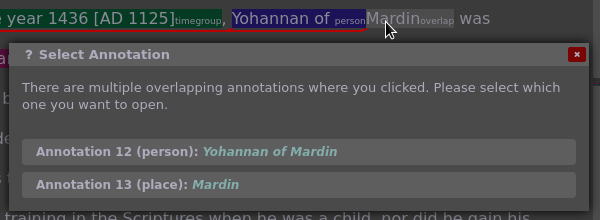
\includegraphics[width=8cm]{../src/assets/annotator-documentation/select-annotation.png}
  \caption{
    When clicking on an overlap between two or more annotations, a pop-up window appears, where you can select which annotation you meant to click on.
  }
  \label{fig:annotation-selection}
\end{figure}

Selecting an annotation is as simple as clicking on it in the document area.
When hovering over the annotation with the mouse, it is already outlined.
Especially in cases where annotations are very long, or there are overlaps with other annotations, this outline can be helpful for understanding which annotation is currently under the mouse cursor.
When annotations overlap and you click on the gray section (i.e., the overlapping part), it is not immediately clear which annotation you want to select.
In that case, a pop-up window appears, listing the different annotation candidates with their type and content (see \cref{fig:annotation-selection}).
By clicking on the intended annotation in the list here, it is selected.
The selection process can be cancelled by clicking on the red cross, or anywhere outside of the pop-up window.


\subsubsection{Editing an Annotation}
\label{sec:annotation-editing}

\begin{figure}[htb]
  \centering
  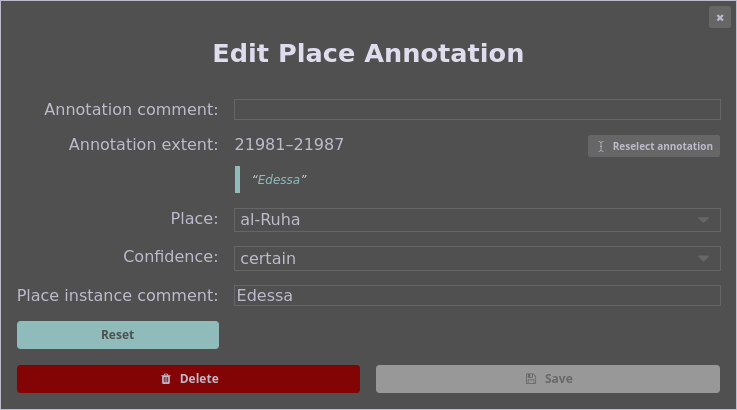
\includegraphics[width=8cm]{../src/assets/annotator-documentation/edit-place-annotation.png}

  \caption{
    The annotation editor for a place annotation.
  }
  \label{fig:edit-place-annotation}
\end{figure}

In the annotation editor, you can edit the \emph{annotation comment,} which is the \verb!comment! field of the record in the \verb!annotation! table.
This might be useful if there is something special about the placement of the annotation in the text, or some useful context.
You can also see and edit the textual extent of the annotation (more details in the next paragraph).
Further, you can edit the \emph{instance} data.
The editors for the different types of annotations, therefore, look slightly different.
\Cref{fig:edit-place-annotation} shows an editor for a place annotation:
Here, the annotation comment field is empty.
For the place instance, the place itself, the location confidence, and the comment in the \verb!place_instance! table can be edited.
The place is selected via a drop-down menu, as is the confidence.
The comments are entered using text fields.
For person and religion annotations, the editors look quite similar, but the first drop-down menu lists persons or religions, respectively.

An annotation has a start and end position in the text, which are stored in the \verb!annotation! table of the database.
As the placement of the annotation could need to be changed, the editors provide a way to see the current extent, and to edit it.
Under the title \emph{\enquote{Annotation extent,}} three elements are visible:
A representation of the start and end position of the annotation, a button to start editing, and a text area where the textual content of the annotation is shown.
To change the extent, click on the button, which is initially labeled \emph{\enquote{Reselect annotation}} (see \cref{fig:edit-place-annotation})
The button now turns red and the text says \emph{\enquote{Cancel}} (see \cref{fig:edit-timegroup-annotation}), and clicking it again will go back to the previous state.
By now selecting a text passage in the document area, the textual extent of the annotation will be updated.
As with all other attributes of the annotation and instance, the changes will only be put into the database when clicking on the save button.
The annotation's textual extent can only be edited for existing annotations, and therefore this facility is not displayed when creating a new annotation.

\begin{figure}[htb]
  \centering
  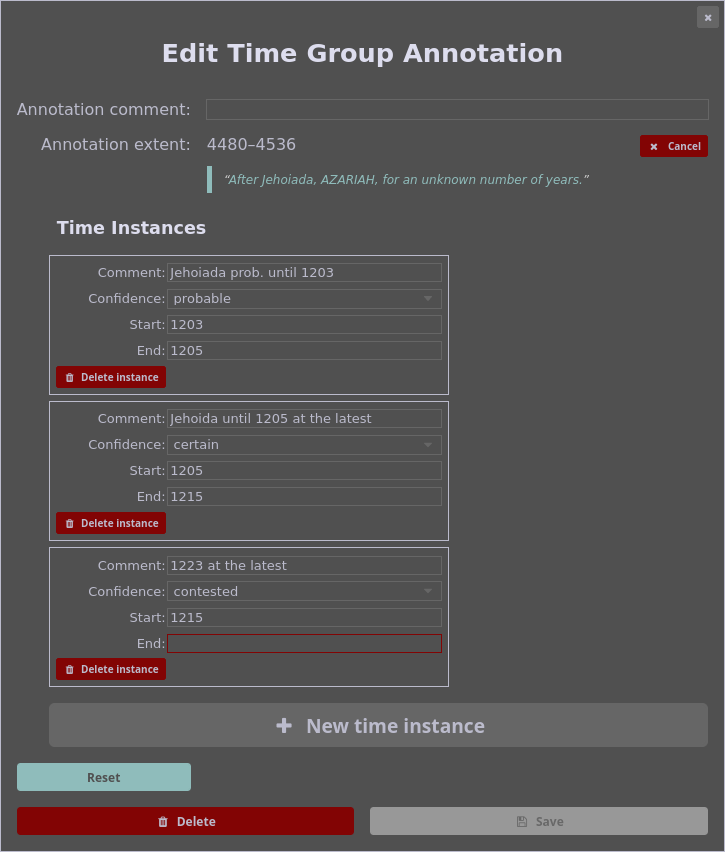
\includegraphics[width=8cm]{../src/assets/annotator-documentation/edit-timegroup-annotation.png}
  \caption{
    The annotation editor for a time group annotation.
    For the third time instance, the mandatory end time field is empty, and the input is therefore outlined in red.
    The user is currently editing the textual extent of the annotation, and the button in that section of the editor therefore reads \emph{\enquote{Cancel.}}
  }
  \label{fig:edit-timegroup-annotation}
\end{figure}

For the time group annotations, the editor looks a bit different because of the way time groups work:
One time group can have zero or more time instances, and all of them would be attributed to the annotation.
\Cref{fig:edit-timegroup-annotation} shows an editor for a time group annotation.
Besides the annotation comment and textual extent, time instances are shown as separate items, where the comment, confidence, start time, and end time can be edited.
In this case, start and end time must be numbers, and the end time must be greater than or equal to the start time.
Each time instance can separately be removed by clicking on the \emph{\enquote{Delete instance}} button in the respective box, and new time instances can be added via the large \emph{\enquote{New time instance}} button.
All changes, additions and deletions are only persisted to the database when the entire time group annotation is saved with the save button in the lower right, and are not persisted if the editor is closed, discarding the edits.

Clicking on the \emph{reset} button in the lower left of the editor will revert the values to their initial state, as if the editor was freshly opened.
The editor can be closed by clicking on the cross in the upper right.
If there are unsaved changes, a prompt will appear to confirm that those changes should be discarded.
The green \emph{save} button in the lower right will persist all changes to the database.
The button will be greyed out and disabled if there are no changes to the annotation yet.
The red \emph{delete} button will delete the instance and annotation (see \cref{sec:annotation-deletion}).

All form data in the editor is validated.
If a field is empty \emph{and} mandatory (e.g., no place is selected for a new place annotation), the field will be outlined in red to signify that.
Similarly, if the content of an input field is invalid (e.g., end time before start time for a time instance), it will be outlined in red as well.
In both cases, the save or create button will be disabled and greyed out.


\subsubsection{Deleting an Annotation}
\label{sec:annotation-deletion}

\begin{figure}[htb]
  \centering
  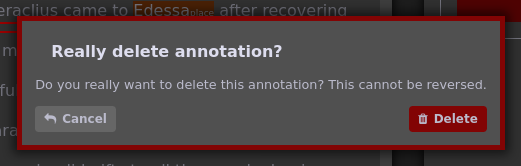
\includegraphics[width=8cm]{../src/assets/annotator-documentation/delete-annotation.png}

  \caption{
    A confirmation dialog appears when deleting an annotation.
  }
  \label{fig:delete-annotation}
\end{figure}

The red \emph{delete} button in the bottom left of the annotation editor will delete the instance and annotation.
Deleting an instance is only possible if the instance is not part of an evidence, and therefore this button is greyed out and disabled if that is the case.
When clicking on the button, a confirmation dialog will first appear to make sure that this is the intended action, see \cref{fig:delete-annotation}.
When clicking \emph{cancel,} the deletion is not performed.
When clicking \emph{delete,} the annotation and the instance will be removed from the database, and the annotation will disappear from the document area.


\subsection{Evidences}
\label{sec:annotator-evidences}

An \emph{evidence,} in general, is a grouping of a \emph{place instance,} a \emph{religion instance,} and optionally a \emph{person instance} and a \emph{time group} (see \cref{sec:database-schema}).
In addition, the evidence has a comment field, the \emph{interpretation confidence} which specifies how confident you are in the interpretation of the source when creating the evidence, and a visibility flag that controls whether the evidence will appear in the visualization or not.

Each evidence also has a \emph{source instance,} which for annotator-generated evidences is created automatically based on the document's source.
Here, the \emph{source confidence,} which specifies the source's trustworthiness for that specific evidence, can also be set.
Last, evidences can be \emph{tagged} with zero or more tags.


\subsubsection{Selecting an Evidence}
\label{sec:evidence-selection}

\begin{figure}[htb]
  \centering
  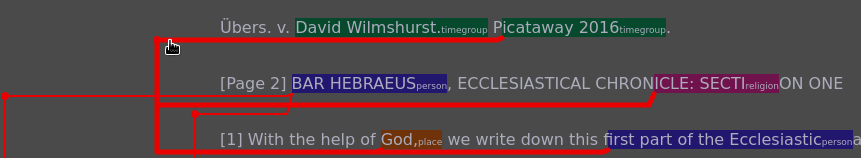
\includegraphics[width=430pt]{../src/assets/annotator-documentation/select-evidence-1.png}\\
  \vspace{10pt}
  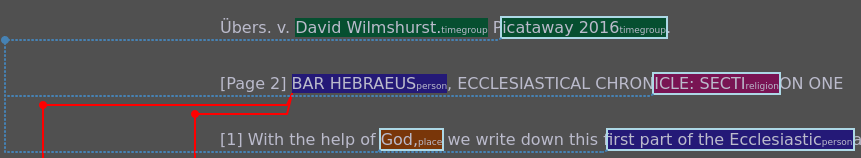
\includegraphics[width=430pt]{../src/assets/annotator-documentation/select-evidence-2.png}

  \caption{
    To select an evidence, hover on the link with the mouse.
    This will already make the link bolder.
    Then clicking the link will select the evidence.
    The link will then turn blue and start to be animated, and the contained annotations are also outlined and animated.
  }
  \label{fig:select-evidence}
\end{figure}

When selecting an evidence, it is opened in the evidence editor.
When creating a new evidence, that new evidence is automatically selected for as long as it is edited.
An existing evidence is selected by clicking anywhere on the link.
The links are layed out in a way that they overlap as little as possible.
To further distinguish which evidence is currently under the cursor, the link gets bolder when the mouse hovers on it.
Clicking on a link will \emph{select} that evidence.
It is then opened in the evidence editor.
Further, the evidence link and the connected annotations are highlighted differently, with blue color and animation, as shown in \cref{fig:select-evidence}.
Selecting a different evidence while the editor is opened will switch to editing that evidence;
however, if there are unsaved changes, a confirmation prompt is shown first.


\subsubsection{Creating an Evidence}
\label{sec:evidence-creation}

\begin{figure}[htb]
  \centering
  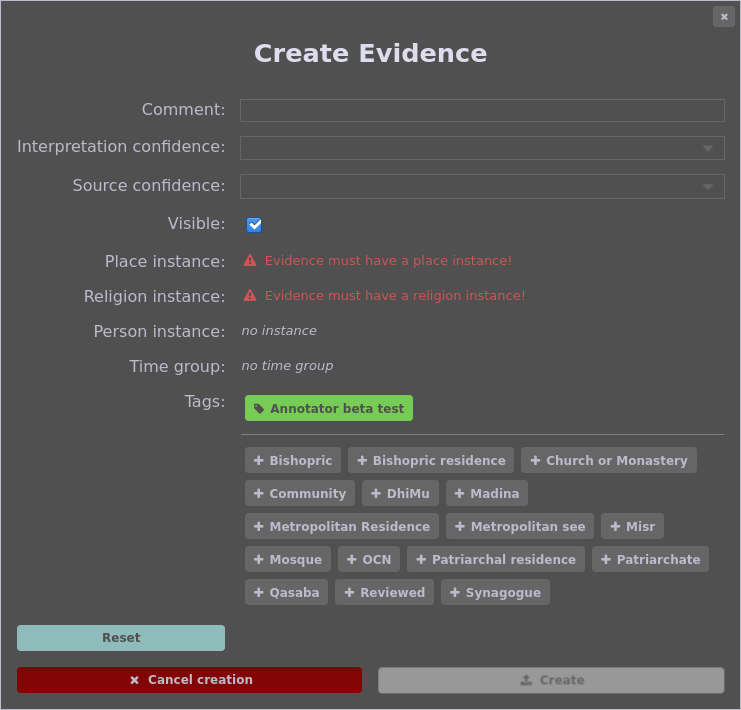
\includegraphics[width=8cm]{../src/assets/annotator-documentation/create-evidence.png}

  \caption{
    Evidence editor for a new evidence.
    The mandatory place and religion instances are empty, and the evidence can therefore not be created yet.
  }
  \label{fig:create-evidence}
\end{figure}

To create an evidence, simply click on the \emph{\enquote{New evidence}} button in the top right of the document area (see \cref{fig:annotator-interface}).
This will open the evidence editor with a new evidence (see \cref{fig:create-evidence}).
While the evidence editor is opened, the button is greyed out and disabled.
As with annotations, creating a new or editing an existing evidence is very similar, and so the description of the editor itself is described below, in \cref{sec:evidence-editing}.
And again, there are slight differences in the three buttons (compare also \cref{fig:create-evidence} and \cref{fig:edit-evidence}).

\begin{enumerate}
  \item the button for closing the editor will cancel creation without a prompt,
  \item the delete button at the bottom is instead labeled \emph{\enquote{Cancel creation}} and serves the same function, and
  \item the save button at the bottom is instead labeled \emph{\enquote{Create}} and clicking it will persist the new evidence to the database.
\end{enumerate}


\subsubsection{Editing an Evidence}
\label{sec:evidence-editing}

\begin{figure}[htb]
  \centering
  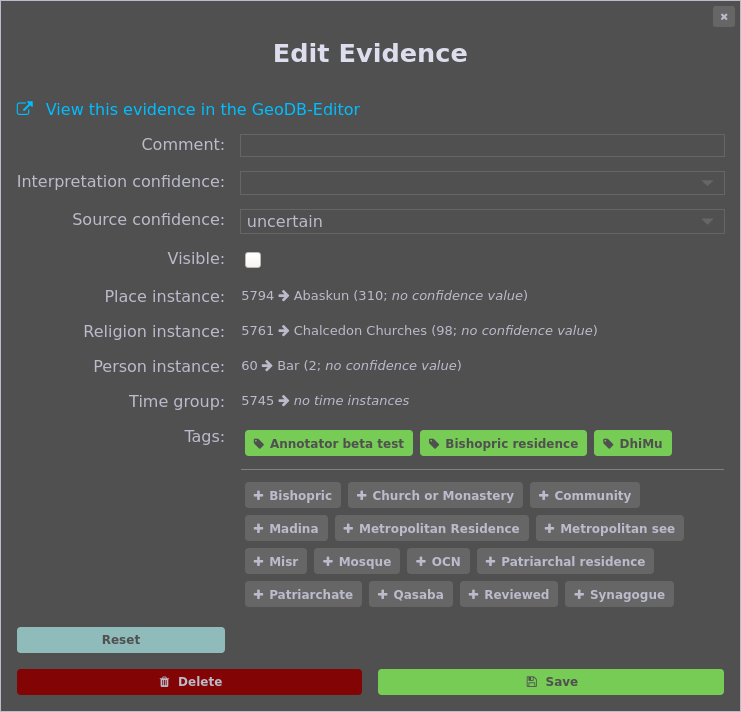
\includegraphics[width=8cm]{../src/assets/annotator-documentation/edit-evidence.png}

  \caption{Evidence editor for an existing evidence.}
  \label{fig:edit-evidence}
\end{figure}

The evidence editor, shown in \cref{fig:create-evidence} and \cref{fig:edit-evidence}, contains four traditional form fields, which are all optional.
These form fields can be edited in a straightforward manner:

\begin{itemize}
  \item a text field for the \verb!comment! field of the evidence,
  \item a drop-down menu for the evidence's \emph{interpretation confidence,}
  \item a drop-down menu for the source instance's \emph{source confidence,} and
  \item a checkbox to toggle the visibility of the evidence in the visualization\footnote{
      Evidence tuples that do not have the \texttt{visible} flag set are \emph{never loaded} from the database.
      While most other filters in the visualization will hide or show evidence dynamically, evidences that are not \emph{visible} will never show up.
      Of course, the visibility can be changed later.
    }.
\end{itemize}

\begin{figure}[htb]
  \centering
  \begin{tikzpicture}
    \node [inner sep=0.0pt,anchor=north west] at (0.5pt,-0.5pt) {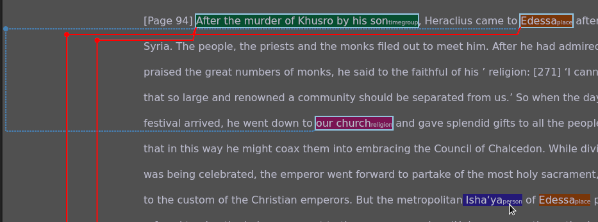
\includegraphics[width=299.0pt,height=111.0pt]{../src/assets/annotator-documentation/evidence-edit-membership-1.png}};
    \node [inner sep=0.0pt,anchor=north west] at (0.5pt,-127.0pt) {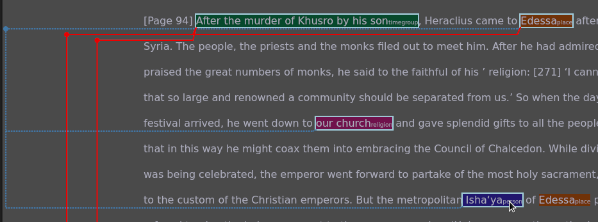
\includegraphics[width=299.0pt,height=111.0pt]{../src/assets/annotator-documentation/evidence-edit-membership-2.png}};

    \begin{scope}[xshift=150.0pt,yshift=-119.0pt,rotate=-90]
      \draw [fill=cyan!80!white!60!black,draw=none] (6.25pt,0.0pt) -- ++(-7.5pt,7.5pt) -- ++(0.0pt,-3.75pt) -- ++(-5.0pt,0.0pt) -- ++(0.0pt,-7.5pt) -- ++(5.0pt,0.0pt) -- ++(0.0pt,-3.75pt) -- cycle;
    \end{scope}

    \draw (227.5pt,-120.0pt)
      node [anchor=east] {\footnotesize Click}
      [red!60!white,-Circle]
      -- ++(10.0pt,0.0pt)
      -- (252.5pt,-105.0pt);
  \end{tikzpicture}

  \caption{
    To toggle membership of an annotation, and its associated \emph{instance,} to an evidence, click on the annotation while the evidence editor is opened.
    The link representing the evidence will update instantly.
  }
  \label{fig:edit-evidence-membership}
\end{figure}

The next four rows represent the place instance, religion instance, person instance, and time group that are part of the evidence.
Here, as the place and religion instance are mandatory, these will show up as red when empty (see \cref{fig:create-evidence}).
These four fields cannot be directly edited (i.e., by clicking or typing in them), but instead are controlled via the \emph{document area.}
While the editor is opened, the annotations that are part of the evidence are outlined in blue and animated.
Changing membership of annotations works as follows (see also \cref{fig:edit-evidence-membership}):
To add an annotation and its instance to the evidence, \emph{click} on the annotation.
To remove an annotation and its instance that are already part of the evidence, also \emph{click} on the annotation (clicking \emph{toggles} membership).
If the evidence already contains an instance and annotation of a certain type, clicking on a \emph{different} annotation of that type \emph{replaces} the previous instance and annotation with the new ones;
for example, if there are two place annotations in the text, one for \textbf{Edessa} and one for \textbf{Damascus,} with \textbf{Edessa} being part of the evidence, clicking on the \textbf{Damascus} annotation would replace the place instance in the evidence, and the evidence would now be related to the place Damascus.
An instance and annotation can be associated with multiple evidences.

The fields in the editor displaying the instances cannot be interacted with directly.
They show more information on the instances themselves and update automatically.
In particular, they show the instance ID, the name and ID of the entity the instance refers to (place, religion, or person), and the respective instance confidence.
For the time group, a comma-separated list of all time instances, with start time, end time, and confidence is shown instead.
The data about the instances must be fetched from the database when it changes, so directly after opening the editor, or when toggling membership of an annotation and instance, the data is not available for a short while, and a loading indicator is shown instead.

If no instance of that type is connected, this is indicated instead, as shown in \cref{fig:create-evidence}.
As the place and religion instances are mandatory, the absence of those is highlighted in red with more urgency.

The last part of the evidence editor is the evidence tags.
Evidence can be tagged to create specific groups of evidences;
for example, evidences that refer to Bishopric residences, or evidences that have been thoroughly reviewed.
An evidence can have zero or more tags.
Tags that are associated with the evidence are displayed at the top in green, tags that are not are displayed below in grey, with a \emph{plus} symbol instead of the \emph{tag} symbol.
To remove an associated tag, click on it, and it moves to the bottom.
Similarly, to add a tag, click on it, and it moves up and becomes green.

As with the annotation editor, all changes made are only local until you click the \emph{save} button at the bottom (or, for new evidences, the \emph{create} button).
Using the \emph{reset} button, the initial state from the database can be restored for all fields, discarding all changes.
Clicking on the cross in the top right closes the editor if there are no unsaved changes, otherwise a confirmation prompt is shown first.
The same prompt is also shown when trying to open a different evidence by clicking on the respective link in the document area.
The \emph{delete} button deletes the evidence, see \cref{sec:evidence-deletion}.
The \emph{save} button will persist all changes to the database.
This button will only be enabled if it is currently possible to save:
If there are no changes, it is disabled and greyed out.
Further, if there is invalid input (i.e., no place or religion instance selected), saving is also not possible.

For evidence that is already saved in the database (i.e., when editing evidence, but not during creation), the evidence editor also shows a link at the top labeled \emph{\enquote{View this evidence in the GeoDB-Editor.}}
Clicking this link will open the GeoDB-Editor, and there select the place of the evidence, scroll down to the evidence table, and select the evidence there as well.
For evidence created using the annotator, a similar link exists in the evidence table of the GeoDB-Editor, which opens the appropriate document in the annotator and opens the respective evidence in the evidence editor.


\subsubsection{Deleting an Evidence}
\label{sec:evidence-deletion}

\begin{figure}[htb]
  \centering
  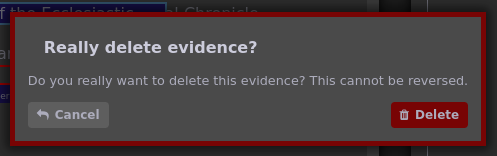
\includegraphics[width=8cm]{../src/assets/annotator-documentation/delete-evidence.png}

  \caption{A confirmation dialog appears when deleting an evidence.}
  \label{fig:delete-evidence}
\end{figure}

Clicking on the red \emph{delete} button in the evidence editor will delete the evidence from the database.
A confirmation dialog (see \cref{fig:delete-evidence}) will appear first to avoid accidental deletions.
In the case of new evidences that have not been saved yet, the button will instead be labeled \emph{\enquote{Cancel creation.}}

Deleting an evidence will \emph{not} delete the connected annotations and instances.
Those will remain in the database and the document area.
It will only delete the evidence itself, the source instance, and all tag associations.
The deletion will be reflected at once in the document area, where the respective link will also disappear.
After deletion, the evidence editor is closed.


\section{Place URI Page}
\label{sec:place-uri-page}

\todo[inline]{todo}

\section{Reporting}
\label{sec:reporting}

Damast provides the option to generate a \emph{report} from a specific subset of historical evidence.
This subset is derived from
\begin{enumerate*}[label=(\arabic*)]
  \item the data contained in the database, and
  \item a set of \emph{filters} concerning different attributes of that data.
\end{enumerate*}
The format and options of these filters are formalized as JSONSchema, and they are a part of the visualization state (see~\cref{sec:vis-reproducible}).
An appropriate file of filters can be obtained (downloaded) from the settings pane of the visualization, or from an existing report.
Report generation can also be triggered directly from the visualization, in which case the state is passed to the report generation software behind the scenes.
In both cases, the filters used are those that are currently active in the visualization as well, meaning that the report will contain the evidences currently shown in the visualization.

The report consists of multiple sections.
First, metadata about the report, such as who provisioned it and when, as well as a textual description of the filters applied within the report, and the cardinality of data entities matching these filters.
Then, the evidences are listed, and their contents are represented as serialized texts.
The entities contained in these evidences (places, religions, and persons) are then listed individually with the relevant information (such as alternative names for the places), and an overall timeline is shown.
Finally, all sources these evidences were extracted from are listed.

All information in the individual sections is cross-referenced.
So, there is a reference from an evidence mentioning a place to the entry for that place in the report;
and vice versa, the places, religions, and persons reference all evidences they are mentioned in.
Further, sources are referenced from the evidences, and the evidences are again referenced as a list from the source section.

In the section of places, the report also shows a map where they are all marked together with the religions mentioned in those places.
This map is generated using \verb!matplotlib!~\cite{Hunter_2007} and is saved both as an SVG file for the HTML version of the report, and as a standalone PDF document for the PDF version.
The PDF map is also stored separately for download.
The map uses Natural Earth~\footnote{\url{https://www.naturalearthdata.com}} vector map data, which is licensed under CC0 (public domain).


\subsection{Generating a Report}
\label{sec:report-generation}
\label{sec:report-lifecycle}

\begin{figure}[tbp]
  \centering
  \includegraphics[]{report-lifecycle/lifecycle.pdf}

  \caption{
    The lifecycle of report records in the database.
    After a report gets provisioned, it is in \texttt{started} state while the report generation code runs.
    If that fails, it enters \texttt{failed} state, otherwise it is \texttt{completed}.
    After a while of not being accessed, the finished report is \texttt{evicted} and only the filter and metadata remain.
    On the next access, the report contents are re-generated from the database.
  }
  \label{fig:report-lifecycle}
\end{figure}


Reports are generated by a separate process within the Docker container that is launched by the server.
\Cref{fig:report-lifecycle} shows the lifecycle of reports.
First, the Flask server generates a UUID for the report; and writes that, the metadata, and the filter into the report database.
At that point, the state of the report is \verb!started!.
Then, it launches the report generation process, passing it the UUID.
The report generation process then reads the filter from the database, collects the data from the PostgreSQL database, and generates the report content.
The content is put together via Jinja2 templates into a HTML page~(\cref{sec:report-html}) and a \TeX{} file, the latter of which is is then compiled into a PDF file~(\cref{sec:report-pdf}).

Once the contents are generated, they are GZIP-compressed and written back into the SQLite3 database.
The state of the report is then set to \verb!completed!.
If an error occurs during report generation, instead an error message is written to the HTML file content in the SQLite3 database, and the state is set to \verb!failed!.

The report contents can be several megabytes large, depending on the number of evidences contained.
To limit storage space requirements on long-running installations, it might be desirable to clean up old, unused reports.
This can always be done from the outside, for example with a \verb!cron(8)! job, working directly with the SQLite3 database.
However, this might not be an ideal solution if generated reports should be guaranteed to persist.
For this, the special \verb!evicted! report state exists, into which a report can be moved.
In that state, the filters and metadata remain in the database, but the report contents are deleted.
The next access to that report then trigger the re-generation of the report\footnote{%
  \textbf{Important note} about report eviction:
  If the goal is to guarantee that reports are always recallable in that state, two other things need to be guarantee on that system:
  \begin{enumerate*}[label=(\arabic*)]
    \item The software version of the Damast system (or at least the report generation software and templates) must not change, and
    \item the contents of the underlying PostgreSQL database must not change.
  \end{enumerate*}
}, and move it back to the \verb!started! state.
Report eviction can also be done manually by setting the content fields to \verb!NULL! in the SQLite3 database, and the \verb!state! field's value to \verb!'evicted'!.
There is also the option to configure the Damast system to handle this automatically via two environment variables:

\begin{description}
  \item[\texttt{DAMAST\_REPORT\_EVICTION\_DEFERRAL}:]
    If this variable exists and is not empty, it specifies a number in days.
    A report is moved to the \texttt{evicted} state if it has not been \emph{accessed}\footnote{%
      Note that eviction deferral does not consider the time since the \emph{creation} of the report, but rather the time since its \emph{last access.}
      Reports might be generated and never again accessed, but they might also be accessed on regular basis, in which case eviction would be deferred.
    } for at least that many days.
    A good number of days to set here could be 90 (three months).
  \item[\texttt{DAMAST\_REPORT\_EVICTION\_MAXSIZE}:]
    If this variable exists and is not empty, it specifies a file size number in \emph{megabytes}.
    The server then regularly checks whether the sum of report content sizes exceeds that size.
    If so, it will evict the least-accessed reports until that sum is less than that size.
    A good number to specify here could be 5,000 (5\,GB).
\end{description}


\subsection{Accessing a Report}
\label{sec:report-access}

Existing reports can be accessed via their UUID.
When generating a report, the user is redirected to the URL where the HTML report (\cref{sec:report-html}) is later shown.
While the report is in \verb!started! state, a wait page is shown that reloads automatically from time to time.
In \verb!failed! state, the error message is shown, and in \verb!evicted! state, opening the page triggers re-generation of the report, and the \verb!started! state's wait page is shown again.
Separate links exist to the PDF version of the report (\cref{sec:report-pdf}) and the standalone map.
All links require knowledge of the report UUID, or access via the list of exiting reports (\cref{sec:report-list}).


\subsection{HTML Report}
\label{sec:report-html}

The HTML report is rendered from a HTML Jinja2 template, which in turn uses many smaller templates and macros to create the contents.
The HTML report content stored in the SQLite3 database is rendered on demand into a template in the website hosted by Damast.
Besides its contents, it contains links to the PDF version, the standalone map, the filters used, a trigger to re-generate the report now, and a link to the visualization, which is then opened with these filters active.


\subsection{PDF Report}
\label{sec:report-pdf}

The PDF report is generated using \LaTeX{}, specifically \XeLaTeX.
In a first step, the \TeX{} code is rendered from a Jinja2 template, which in turn uses many smaller templates and macros to create the contents.
The \verb!latexmk! utility is then used to compile the \TeX{} code within the Docker container.
The resulting PDF file is stored into the SQLite3 database.
Accessing the PDF file\footnote{Via \texttt{\$\{DAMAST\_PROXY\_PREFIX\}/reporting/<uuid>/pdf}} then offers the PDF file for download.
The PDF version of the map is used in the PDF report and compiled into it by \XeLaTeX{}.
It can also be downloaded separately\footnote{Via \texttt{\$\{DAMAST\_PROXY\_PREFIX\}/reporting/<uuid>/map}}.


\subsection{List of Reports}
\label{sec:report-list}

In the miscellaneous pages (see~\cref{sec:other-pages}), a page that lists existing reports is also available.
Users with the \verb!admin! role see all reports in the database, other users only see their own.
However, this page only exists for users that are logged in, not for anonymous visitors.
This is because visitors (if they have the \verb!reporting! role) all generate reports under the \verb!visitor! pseudo-user, and there is no way to determine which reports a visitor has provisioned.

The list shows the user, UUID, server version, start time, run duration, and number of evidences.
Further, there are links to the HTML and PDF versions, the standalone PDF map, and the filter file.
Another link will trigger report re-generation with the same filters\footnote{%
  This will create a \emph{new} report and UUID.
  Note that this does not make sense on a system where the PostgreSQL database contents never change.
  }.
Lastly, a link to the visualization will open that with the filters of that report active.


\section{Other Pages}
\label{sec:other-pages}

A few other, miscellaneous pages exist on the \verb!docs! blueprint.
These also include an index page under \verb!${DAMAST_PROXY_PREFIX}/docs/! that shows links to all of these pages that the user is allowed to visit.

\subsection{Documents}

The documents page contains links to a few smaller pages and utilities.
Some of these are not available to all users, but only to developers or administrators.
Besides the page links listed in the following, the documents page also has links to the report creation page and the list of existing reports detailed in \cref{sec:reporting}.

\paragraph*{Database edit log.}
This page is visible only to administrators (role \verb!admin!).
It details the contents of the \verb!user_action! table in reverse chronological format.
This data can be reviewed for provenance, or to quickly retrieve an old value from a database entry after a mistake in an edit.

\paragraph*{REST API documentation.}
This page is visible to all developers (role \verb!dev!), and contains a list of the endpoints in the REST API (see~\cref{sec:rest-api}).
They are the HTTP endpoints under \verb!/rest/!, which are listed in the form they are defined in Flask.
The URL and possible HTTP verbs are extracted from Flask runtime information, and the documentation string is taken directly from the Python \emph{docstring} of that method.
The REST API methods' docstring are all quite detailed and show request and response content types, possible values and data entries, and payload or response examples, where applicable.

\paragraph*{Annotator user guide.}
The annotator user guide explains how the annotator works and is used in great detail, and with example images.
This page is visible to all users with the \verb!annotator! role.
The annotator user guide is the basis for the text in \cref{sec:annotator}.

\paragraph*{PostgreSQL Database Schema.}
Download link to a PDF of the database structure.
This link is available to all developers (role \verb!dev!) and to users with the \verb!pgadmin! role.
The PDF is the same as \cref{fig:db-structure}, enclosed in a page with headers and footers.

\paragraph*{Download database dump.}
Download link to a SQL dump of the entire database.
The file is served as GZIP-ed SQL, and is generated on the fly.
This functionality is available to all users.
However, if the requesting user does \emph{not} have the \verb!admin! role, the dump is data-only, and also omits the \verb!action_type!, \verb!user!, and \verb!user_action! provenance tables described in \cref{sec:provenance-tables}.


\subsection{GDPR, Imprint, Cookie Preferences}

A separate blueprint serves pages for the GDPR\footnote{
  \textbf{GDPR:} General Data Protection Regulation of the European Union.
  Called DSGVO \emph{(Datenschutzgrundverordnung)} in German.
}
content.
These pages are accessible even without login, and are available as links in the footer of each page\footnote{
  In the visualization, which has a tighter layout without a footer, these links are placed in the header instead.
}.
A general data protection page states what data is collected from visitors, and what rights they have under GDPR.
The imprint \emph{(Impressum)} page contains information about how to get in touch with the website administrators.
Finally, the websites use cookies and \verb!localStorage! to store state and information on the user's computer.
These are used for login, but also for functionalities such as storing table or visualization layout.
In accordance to \S\,7 \P\,2 GDPR, consent to store these cookies needs to be given explicitly by users.
For this, they are shown a consent popup when they first visit the site, with the choices of
\begin{enumerate*}[label=(\arabic*)]
  \item no cookies,
  \item only necessary cookies, or
  \item all cookies.
\end{enumerate*}
Users must be able to amend or withdraw consent at any time (\S\,7 \P\,3 GDPR), so the consent settings shown in the popup are also available as a separate page.

Users must consent to necessary cookies (option (2)) to be able to login, as the session cookie must be stored.
Further, the consent itself is stored as a cookie.
Consequently, visitors who reject all cookies (option (1)) will be shown the cookie consent popup each time they open a page, as there is no way to store their choice.
The \enquote{all cookies} option (3) is necessary to use additional features such as storing custom visualization and table layouts.

When hosting the Damast system somewhere else, a different imprint than the default one is needed if the administrators and hosting organization differ.
Probably, the data protection page needs to be modified as well.
Here, the blueprint override functionality discussed in \cref{sec:override-blueprints} can come in handy.


\subsection{Login and Password Management}

A blueprint provides login and logout functionality, as well as a page to change the current user's password.
These are linked in the top right of the page, in the header.
If a visitor is not logged in, a link to the login page is shown there.
If they are logged in, the user's name, a link to the password change page and a link to log out is shown.

On the password change page, the user must enter their current and their new password, and then submit.
The server backend will check that the old password matches, and that the new password has sufficient complexity (entropy).
If that is the case, the password hash is updated in the user database and the session token is renewed.
